% !TEX TS-program = XeLaTeX
\documentclass[11pt]{article}

% Packages
\usepackage[margin=1in]{geometry}
\usepackage{fancyhdr}
\usepackage{iftex}
\ifPDFTeX
  \usepackage[T1]{fontenc}
  \usepackage{lmodern}
  \DeclareRobustCommand{\ph}[1]{#1}
  \DeclareRobustCommand{\phA}{A}
\else
  \usepackage{fontspec}
  \IfFontExistsTF{Noto Sans Phoenician}{
    \newfontfamily\phoenicianfont{Noto Sans Phoenician}
    \DeclareRobustCommand{\ph}[1]{\ifmmode\text{\phoenicianfont #1}\else{\phoenicianfont #1}\fi}
    \DeclareRobustCommand{\phA}{\ph{\char"10900}} % Aleph
  }{
    \DeclareRobustCommand{\ph}[1]{#1}
    \DeclareRobustCommand{\phA}{A}
  }
\fi
\usepackage{microtype}
\usepackage[round]{natbib}
\usepackage[hidelinks]{hyperref}
\usepackage{bookmark}
\usepackage{graphicx}
\usepackage{booktabs}
\usepackage{amsmath, amssymb, amsfonts}
\usepackage{dsfont}
\usepackage{xcolor}
\usepackage{siunitx}
\usepackage[nameinlink,noabbrev]{cleveref}
\usepackage{enumitem}
\usepackage{float}

% TikZ
\usepackage{tikz}
\usepackage{pgfplots}
\pgfplotsset{compat=1.18}
\usetikzlibrary{
  arrows.meta,
  positioning,
  shapes.geometric,
  shapes.misc,
  calc,
  fit,
  backgrounds
}

% Algorithms
\usepackage{algorithm}
\usepackage{algpseudocode}

% Figures / captions
\usepackage{caption}
\usepackage{subcaption}

\setcounter{tocdepth}{2}

% Formatting
\setlength{\parindent}{0pt}

% Consistent paragraph spacing
\setlength{\parskip}{0.6ex} % match the visual gap

% Macros
\newcommand{\TODO}[1]{\textcolor{red}{[\textbf{TODO:} #1]}}
\newcommand{\act}[1]{\texttt{#1}}
\newcommand{\canvas}[1]{\texttt{#1}}

\DeclareRobustCommand{\Stop}{\ifmmode\text{\textsc{Stop}}\else\textsc{Stop}\fi}
\DeclareRobustCommand{\Insert}{\ifmmode\text{\textsc{Insert}}\else\textsc{Insert}\fi}
\DeclareRobustCommand{\Ins}{\Insert}
\DeclareRobustCommand{\Move}{\ifmmode\text{\textsc{Move}}\else\textsc{Move}\fi}

\DeclareRobustCommand{\Delete}{\ifmmode\text{\textsc{Delete}}\else\textsc{Delete}\fi}
\DeclareRobustCommand{\Del}{\Delete}
\DeclareRobustCommand{\Replace}{\ifmmode\text{\textsc{Replace}}\else\textsc{Replace}\fi}
\DeclareRobustCommand{\SpanDelete}{\ifmmode\text{\textsc{SpanDelete}}\else\textsc{SpanDelete}\fi}
\DeclareRobustCommand{\Swap}{\ifmmode\text{\textsc{Swap}}\else\textsc{Swap}\fi}
\DeclareRobustCommand{\SpanMove}{\ifmmode\text{\textsc{SpanMove}}\else\textsc{SpanMove}\fi}
\DeclareRobustCommand{\SpanCopy}{\ifmmode\text{\textsc{SpanCopy}}\else\textsc{SpanCopy}\fi}

% Common symbols
\newcommand{\Mset}{\mathcal{M}}
\newcommand{\clip}{\mathrm{clip}}

% Push floats to top on float-only pages
\makeatletter
\setlength{\@fptop}{0pt}
\setlength{\@fpsep}{10pt}
\setlength{\@fpbot}{0pt plus 1fil}
\makeatother
\renewcommand{\topfraction}{0.95}
\renewcommand{\textfraction}{0.05}
\renewcommand{\floatpagefraction}{0.80}

% siunitx setup
\sisetup{
  detect-all,
  group-separator = {,},
  group-minimum-digits = 4,
  round-mode = places,
  round-precision = 2
}

\definecolor{TokGreen}{HTML}{1B7F3A} % dark-ish green
\definecolor{TokRed}{HTML}{B3261E}   % dark-ish red

% Figure colors (for reviser-step and trajectory figures)
\definecolor{FigText}{HTML}{222222}
\definecolor{FigTyrianPurple}{HTML}{66023C}
\definecolor{FigBlue}{HTML}{3B82F6}
\definecolor{FigGray}{HTML}{E5E7EB}
\definecolor{FigDarkGray}{HTML}{6B7280}
\definecolor{FigLightBlue}{HTML}{DBEAFE}
\definecolor{FigLightOrange}{HTML}{FEF3C7}
\definecolor{FigRed}{HTML}{B91C1C}

% Units (appendix convention: 1 MAC = 1 FLOP unit)
\newcommand{\G}{\mathrm{G}} % billions of MACs
\newcommand{\M}{\mathrm{M}} % millions of MACs

% Token styling (monochrome-friendly)
\newcommand{\TokG}[1]{\begingroup\color{TokGreen}\ifmmode #1\else\texttt{#1}\fi\endgroup}
\newcommand{\TokR}[1]{\begingroup\color{TokRed}\ifmmode #1\else\texttt{#1}\fi\endgroup}
\newcommand{\GapR}[1]{\underline{\texttt{<+#1>}}}
\newcommand{\Sep}{\;\,}

% TikZ styles
\tikzset{
  diagramBox/.style={
    draw, thick, rounded corners=2pt,
    align=center,
    inner sep=6pt,
    minimum height=10mm,
    text width=35mm
  },
  diagramSmall/.style={
    draw, thick, rounded corners=2pt,
    align=center,
    inner sep=4pt,
    minimum height=8mm,
    text width=28mm
  },
  diagramArrow/.style={-Latex, thick},
  diagramDashed/.style={draw, thick, dashed, rounded corners=2pt},
  diagramTitle/.style={font=\bfseries},
  stepBox/.style={
    draw, thick, rounded corners=2pt,
    align=left,
    inner sep=5pt,
    text width=115mm
  },
  decision/.style={
    diamond, draw, thick, aspect=2,
    align=center, inner sep=2pt, text width=25mm
  }
}

\usepackage{placeins} % optional float controls (no section barriers used)

% Math symbols, but safe in text contexts (like \item labels)
\newcommand{\reproyes}{\ensuremath{\checkmark}}
\newcommand{\reprono}{\fbox{\rule{0pt}{0.9ex}\rule{0.9ex}{0pt}}}

\newcommand{\ReviserInferMult}{\num{1.394}}

\title{Reviser: Revision-Capable Text Generation via Autoregressive Cursor Actions}
\author{
Sean Diab\\
Independent Researcher\\
\texttt{diabsean2005@gmail.com}
}

\fancypagestyle{firstpage}{
  \fancyhf{}
  \fancyfoot[C]{\footnotesize\shortstack{Code: \url{https://github.com/Sean-Diab/Reviser}\\Checkpoints: \url{https://huggingface.co/sean-diab/reviser-checkpoints}}}
  \renewcommand{\headrulewidth}{0pt}
  \renewcommand{\footrulewidth}{0pt}
}

\begin{document}
\maketitle
\thispagestyle{firstpage}

\begin{abstract}
Revision-capable generation is appealing because it can insert or revise earlier content, but many non-autoregressive and edit-based approaches obtain this flexibility through repeated sequence-level computation. We propose Reviser, a decoder-only Transformer that generates a response as a sequence of cursor-relative actions on a mutable canvas. At each step, Reviser predicts exactly one action token: \Insert(token), \Move($\Delta$), or \Stop, and is autoregressive over edit-history actions rather than final text order.

This design enables genuinely non-monotonic generation while preserving a simple next-action interface. On a continuation benchmark, Reviser is strongly preferred to SEDD and MDLM in our arena evaluations, and trajectory statistics confirm that the model performs frequent backward moves and mid-canvas insertions rather than merely emulating end-append decoding. Against size-matched autoregressive baselines, Reviser is competitive at both the 100M and 300M scales. Under our shared FLOPs convention, Reviser also requires substantially less inference compute than representative multi-pass refinement and diffusion-style baselines.
\end{abstract}

\section{Introduction}
\label{sec:intro}

Autoregressive Transformers dominate text generation, but they are structurally biased toward producing content in final left-to-right order: once a clause is emitted, correcting it typically requires generating additional text after it rather than directly revising earlier content \citep{vaswani2017attention,brown2020language}. Revision-capable and non-autoregressive methods promise post-hoc correction and increased parallelism, yet in practice they frequently incur large overhead in the forms of multiple full-sequence refinement passes, scoring every insertion slot, or many-step sampling procedures \citep{ghazvininejad2019maskpredict,gu2019levenshtein,li2022diffusionlm,lou2024sedd,sahoo2024mdlm}. This paper asks: can we get revision-style generation while keeping total compute close to a standard AR Transformer?

We propose Reviser, which generates by executing a stream of simple cursor edits on a mutable canvas. In the primary implementation, Reviser uses only insert and move actions (plus $\Stop$), where ``revision'' means non-left-to-right insertion into earlier positions; although Reviser naturally supports richer edit operators (e.g., $\textsc{Delete}$/$\textsc{Replace}$/span edits), we focus here on this minimal insert+move (+$\Stop$) instantiation and leave destructive editing to future work. The model is a standard decoder-only transformer, but crucially, it is autoregressive over action tokens (the edit history), not over the final text token order. Because the cursor can move and insert earlier content, Reviser is not constrained to left-to-right generation in the final text order, enabling revision-like behavior while keeping each model call ``normal-sized.''

Rather than outputting a distribution over all positions (or all insertion slots) at each step, Reviser outputs exactly one cursor-relative action token per step. Importantly, the transformer trunk attends only to the action-history sequence $H_t$; it never attends to canvas tokens directly. The canvas is implicit in the history of executed actions and is accessed only through validity masking. This keeps each model call comparable to a standard AR step (transformer trunk + one head). The remaining overhead is the number of action steps, which can be close to the output length in an insert-dominant regime.

Beyond text continuation, the cursor-action formulation also suggests applications to structured editing tasks such as code or document modification. Modern agent systems often edit files by repeatedly proposing diffs or patches over entire sequences \citep{yang2024sweagent,gauthier2024aider}, which can require multiple full-sequence passes. In contrast, Reviser operates through localized insert and move actions on a mutable canvas, which may offer a more natural interface for incremental editing. We do not evaluate this setting in the current work, but view it as a promising direction for future research.

A concrete example helps illustrate the behavior. In one 300M Reviser generated trajectory (300M Reviser Example 1 in ~\Cref{sec:appendix_ranked_examples}):
\begin{quote}
\textbf{Before edit}\\
\ttfamily\small Information is deemed correct and is subject to change. Real estate listings obtained from third party sources are for \textbar{} consumers' personal purchasing decisions and should...
\\[0.25em]
\textbf{Actions (steps 204-209)}\\
\ttfamily\small \textcolor{FigBlue}{\textsc{Move}(-16)} \;+\; \textcolor{FigTyrianPurple}{\textsc{Insert}}(\texttt{at the time of publishing})
\\[0.25em]
\textbf{After move}\\
\ttfamily\small Information is deemed correct at the time of publishing \textbar{} and is subject to change. Real estate listings obtained from third party sources are for...
\end{quote}
This edit makes the statement more precise. \Cref{sec:appendix_ranked_examples} provides full qualitative examples and trajectories.

\paragraph{Contributions.}
\begin{enumerate}[leftmargin=*,itemsep=0.2em]
\item We introduce Reviser, a cursor-action generator that is autoregressive over edit-history actions rather than final text order.
\item We formalize the canvas state, cursor-based edit operators, validity masking, and deterministic executor updates for the insert+move+\Stop{} setting.
\item We describe an obfuscation--restoration supervision scheme for training next-action predictors on edit trajectories.
\item We show empirically that Reviser produces genuinely non-monotonic trajectories, with frequent backward moves and mid-canvas insertions.
\item We evaluate Reviser on continuation against diffusion and autoregressive baselines, and analyze quality, length behavior, and trajectory statistics.
\item We provide an analytic FLOPs-based comparison showing that Reviser is substantially cheaper than representative multi-pass refinement and diffusion-style baselines under a shared convention.
\end{enumerate}

\Cref{sec:setup} states the problem setup and design goals, and \Cref{sec:why_nar_costs} motivates the compute tradeoffs behind our design. \Cref{sec:related} situates Reviser in prior work. Section~\ref{sec:overview}--Section~\ref{sec:model} formalize Reviser and the decoding procedure, and \Cref{sec:training} describes supervision via obfuscation--restoration trajectories. \Cref{sec:experiments} reports empirical results, while \Cref{sec:limitations}--\Cref{sec:conclusion} discuss limitations, future directions, and conclusions. The Appendix provides additional variants, full FLOPs/accounting derivations, qualitative examples, and reproducibility details.

\section{Problem Setup and Design Goals}
\label{sec:setup}

Reviser supports prompt-conditioned generation in general; in this work, we instantiate it as a prefix-seeding text continuation model: given an input prefix $x = (x_1,\dots,x_m)$, the goal is to generate the continuation sequence.

To make the prefix visible to the history-only model, we write it into both the canvas and the action history via a deterministic insert-only prefix-seeding action sequence:
\[
\phA^{\text{pref}}(x) \;=\; \bigl(\Insert(x_1),\,\Insert(x_2),\,\dots,\,\Insert(x_m)\bigr).
\]
Executing $\phA^{\text{pref}}(x)$ from a blank canvas places each prefix token on the canvas in order, sets the cursor at position $m$, and makes the full prefix content visible to the transformer through its action-history input $H_t$. Continuation decoding then begins from this seeded state, with a validity mask that prevents edits to the prefix region.

Our design goal is to support revision-capable generation, the ability to insert or modify earlier content during decoding, while keeping the compute profile close to a standard AR transformer.

We aim to avoid common sources of overhead in prior NAR approaches:
(i) repeated full-sequence refinement passes,
(ii) per-step scoring over all positions/slots,
(iii) large per-position action heads, and
(iv) sampling procedures requiring many denoiser steps.
Reviser instead makes a single cursor-relative decision per step using a standard transformer trunk and a single action head.

We evaluate (a) generation quality (evalPPL under GPT-2 Large and arena pairwise win rates), (b) compute (FLOPs), and (c) trajectory behavior (steps/token, move fraction, cursor travel, insertion locations).

\begin{table}[t]
\centering
\small
\setlength{\tabcolsep}{6pt}
\begin{tabular}{ll}
\toprule
Symbol & Meaning \\
\midrule
$x=(x_1,\dots,x_m)$ & input prefix (conditioning context) \\
$m$ & prefix length in tokens \\
$\phA=(a_1,\dots,a_T)$ & restoration trajectory (total action sequence) \\
$B=(b_1,\dots,b_{n_{\text{obf}}})$ & obfuscation trajectory (action sequence) \\
$V_c$ & insert token vocabulary \\
$V_a$ & action vocabulary ($V_c \cup \Mset \cup \{\Stop\}$) \\
$C_t=(c_{t,1},\dots,c_{t,\ell_t})$ & canvas token sequence at step $t$ \\
$\ell_t$ & canvas length at step $t$ \\
$u_t\in\{0,\dots,\ell_t\}$ & cursor boundary index (between tokens) \\
$H_t$ & edit-history action sequence at continuation step $t$ (includes prefix-seeding actions) \\
$n$ & final token output length (reference; not edit-history length) \\
$p_{\text{move}}$ & fraction of generated actions that are \Move{} actions \\
$n_{\text{eff}}$ & effective action length, $n_{\text{eff}} \triangleq \frac{n}{1-p_{\text{move}}}$ \\
$T_{\text{rest}}$ & restoration trajectory length in actions (including $\Stop$) \\
$T_{\text{dec}}$ & diffusion-style reverse/denoising step count \\
$T_{\text{mp}}$ & Mask-Predict/CMLM refinement-iteration count \\
$F_{\text{mult}}(a,b,c)$ & MAC-count proxy for matmul $[a\times b]\cdot[b\times c]$ \\
$F_{\text{transformer}}^{\text{full}}(n)$ & trunk cost for one full-attention Transformer pass at length $n$ \\
$F_{\text{transformer}}^{\text{causal}}(n)$ & trunk cost for one causal-attention Transformer pass at length $n$ \\
$F_{\text{infer}}^{\mathcal{M}}(n)$ & total inference compute for method $\mathcal{M}$ \\
$I_{\text{infer}}^{\mathcal{M}}$ & inference multiplier vs AR: $F_{\text{infer}}^{\mathcal{M}}/F_{\text{infer}}^{\text{AR}}$ \\
\bottomrule
\end{tabular}
\caption{Notation used throughout the paper (core variables).}
\label{tab:notation}
\end{table}

\section{Compute Tradeoffs in Existing NAR and Edit-Based Transformers}
\label{sec:why_nar_costs}

Many non-autoregressive and edit-based Transformers obtain flexibility or parallelism by repeating expensive sequence-level computation multiple times per response \citep{lee2018deterministic,ghazvininejad2019maskpredict,gu2019levenshtein,li2022diffusionlm,lou2024sedd,sahoo2024mdlm}. Under a shared FLOPs convention, this often leads to substantially higher total inference compute than a standard autoregressive baseline. Our goal in this section is not to claim that all such methods are inefficient in practice, but rather to highlight a common tradeoff: repeated full-sequence prediction can raise total compute even when sequential dependence is reduced.

In our FLOPs accounting (\Cref{app:prior_art_efficiency_flops}), an AR baseline produces a length-$n$ response with one full-sequence evaluation. By contrast, most NAR families run multiple full-sequence evaluations (refinement iterations, insertion rounds, denoising steps, etc.), so they repeatedly pay the dominant Transformer trunk cost over all $n$ positions.

A single full-sequence evaluation computes hidden states for all $n$ positions and then applies a vocab projection, yielding $n\times |V|$ logits. At modern scales, both terms matter: the full Transformer pass is expensive, and the vocab head is also large and non-negligible (e.g., $|V|\approx 50\text{k}$). Methods that perform $R$ refinement/denoising iterations therefore multiply both costs by roughly $R$ per response, often with additional task-specific heads, slot-scoring loops, or auxiliary passes. In several families, $R$ is large: for example, CMLM commonly uses around $R=10$ refinement passes, while diffusion-style decoders often use $R=T_{\text{dec}}\in[200,2000]$ reverse steps. This repeated sequence-level evaluation is highly inefficient at inference time, especially for long outputs or throughput-limited deployment.

For overall efficiency, especially at scale, the dominant quantity is often total FLOPs per response. If a method is $10\times$ more compute-intensive, modest systems-level scheduling gains usually do not offset that gap. Total compute is therefore the primary constraint for training cost, energy, and throughput-limited deployments. We report a compute multiplier
\[
I_{\text{infer}}^{\mathcal{M}} \;\triangleq\; \frac{F_{\text{infer}}^{\mathcal{M}}}{F_{\text{infer}}^{\text{AR}}},
\]
where $F_{\text{infer}}^{\mathcal{M}}$ is the total FLOPs to generate a full length-$n$ response under method $\mathcal{M}$'s decoding procedure. In this section and appendix, we focus on $F_{\text{infer}}^{\mathcal{M}}$ and $I_{\text{infer}}^{\mathcal{M}}$ as the primary compute indicators.

\Cref{tab:prior_art_summary_main} summarizes our computed multipliers relative to the AR baseline (derivations in the Appendix). With few exceptions, popular NAR Transformers require significantly more total compute than AR, often by an order of magnitude or more. The methods that appear closer to AR in compute typically rely on highly parallel, one-/few-shot predictions; in practice these variants struggle due to the parallel decoding issue (below), and are commonly augmented with iterative refinement, which reintroduces the repeated-pass overhead.

The most compute-efficient NAR variants attempt to predict many (or all) output tokens simultaneously.
This creates a global coordination problem: each position must choose a token that is compatible with the (unknown) choices at other positions.
Formally, one-shot NAR variants often behave like a product-of-marginals approximation \citep{gu2018nonautoregressive},
\[
p(y\mid x)\approx \prod_{i=1}^{n} p(y_i\mid x),
\]
which cannot reliably enforce inter-token constraints without extra structure (latents, constraints, or iterative refinement).
In practice, this manifests as agreement errors, repetition, missing required entities, and internal contradictions, motivating additional passes that raise compute.


\begin{table}[tbp]
\centering
\small
\setlength{\tabcolsep}{6pt}
\begin{tabular}{lccc}
\toprule
Method (family / variant) & Decoding structure & $I_{\text{infer}}^{\mathcal{M}}$ & Parallel decoding issue? \\
\midrule
AR (baseline) & $n$ AR steps & \num{1.00} & \TokG{No} \\
Reviser (this work) & $T_{\text{rest}}$ AR-style steps & \num{1.25}--\num{1.50}$^{\dagger}$ & \TokG{No} \\
\midrule
LevT (iterative edit/refine) & $R\in\{5,10\}$ passes & \num{6.91}--\num{19.40} & \TokR{Yes} \\
InsT (balanced-tree) & $\log_2 n$ passes & \num{2.02} & \TokR{Yes} \\
InsT (serial) & $n$ passes & \num{65.01} & \TokG{No} \\
CMLM / Mask-Predict ($T_{\text{mp}}{=}10$) & 10 passes & \num{11.86} & \TokR{Yes} \\
Diffusion-LM ($T_{\text{dec}}{=}200$--$2000$) & 200--2000 passes & \num{140.51}--\num{1402.36} & \TokG{No} \\
\midrule
One-shot NAT (few-pass) & 1 enc + 1 dec pass & \num{1.96} & \TokR{Yes} \\
\bottomrule
\end{tabular}
\caption{Analytic inference-compute summary under a shared FLOPs convention (computed in the Appendix).
$I_{\text{infer}}^{\mathcal{M}} \triangleq F_{\text{infer}}^{\mathcal{M}}/F_{\text{infer}}^{\text{AR}}$ is the total inference FLOPs multiplier of method $\mathcal{M}$ relative to AR; values are structural estimates, not measured wall-clock latency.
$\dagger$~Range shown for $p_{\text{move}}\in\{0.20,0.28,0.33\}$ at $n=128$ (including observed move fractions from \Cref{tab:trajectory_stats}); see \Cref{app:reviser_flops}.
For AR/Reviser, ``steps'' denotes KV-cached next-token/next-action decoding; ``passes'' for other methods denotes repeated full-sequence evaluations.
``Parallel decoding issue'' marks families whose highly parallel variants often underperform due to global coordination constraints, commonly motivating additional refinement passes. Further details of all calculations are provided in \Cref{app:prior_art_efficiency_flops}.}
\label{tab:prior_art_summary_main}
\end{table}

Reviser avoids the parallel-decoding coordination issue by predicting one cursor-relative action token at a time, conditioned on the full prior edit history. This keeps global coherence through autoregressive dependence while still allowing non-monotonic canvas edits. It also avoids repeated full-sequence refinement: each step is a standard AR-style next-action pass, rather than repeated re-evaluation over all $n$ output positions. If the move fraction is $p_{\text{move}}$, producing $n$ final tokens takes an expected $n_{\text{eff}}=\frac{n}{1-p_{\text{move}}}$ action steps, so
\[
I_{\text{infer}}^{\text{Reviser}}(n)\approx\frac{F_{\text{infer}}^{\text{AR}}(n_{\text{eff}})}{F_{\text{infer}}^{\text{AR}}(n)}.
\]
For $p_{\text{move}}\in\{0.20,0.28,0.33\}$ and $n=128$, this gives
$n_{\text{eff}}\in\{160,\;177.78,\;191.04\}$ and
$I_{\text{infer}}^{\text{Reviser}}(128)\in\{\num{1.25},\;\num{1.39},\;\num{1.50}\}$.

\section{Related Work}
\label{sec:related}

Reviser is closest to non-autoregressive and partially autoregressive generation that relaxes strict left-to-right decoding. Early one-shot NAT models improve parallelism but face multimodality and coordination issues \citep{gu2018nonautoregressive}; iterative variants such as deterministic refinement and Mask-Predict improve quality by repeating full-sequence passes \citep{lee2018deterministic,ghazvininejad2019maskpredict}. Reviser targets the same non-monotonic capability, but keeps a one-action interface per step instead of repeated sequence-level prediction.

Our approach is also related to insertion and edit-based generation. Insertion Transformer and Levenshtein Transformer show that insertion/deletion operations can realize flexible generation orders \citep{stern2019insertion,gu2019levenshtein}. Text-edit tagging systems such as LaserTagger and FELIX frame generation as edit prediction over an existing sequence \citep{malmi2019lasertagger,mallinson2020felix}. Many of these methods were introduced and evaluated primarily in sequence transduction settings (especially machine translation and grammatical-error-correction style tasks), rather than open-ended continuation generation. PIE-style post-editing formulations make a similar design choice by treating generation as targeted rewriting rather than pure left-to-right continuation. Reviser is in the same family of ideas, but uses explicit cursor actions with deterministic executor semantics.

Diffusion-style LMs provide another route to non-monotonic generation. Diffusion-LM, SEDD, and MDLM decouple final token order from AR factorization through denoising trajectories \citep{li2022diffusionlm,lou2024sedd,sahoo2024mdlm}. More recent semi-AR or block-diffusion variants, including LLaDA, Dream, and SDLM (analyzed in our Appendix FLOPs section), further explore the quality and throughput tradeoff by mixing iterative denoising with partial autoregressive structure.

Latent-variable NAR models are also relevant. Flow-based sequence generators such as FlowSeq model conditional generation through invertible latent transformations instead of strict tokenwise AR decoding \citep{ma2019flowseq}. This line is conceptually close in its goal of relaxing left-to-right constraints, though its modeling interface differs from explicit executable edit actions.

Reviser also relates to work on non-left-to-right autoregression. XLNet demonstrates permutation-based autoregressive objectives over factorization orders \citep{yang2019xlnet}, and insertion-based AR models similarly depart from fixed final-token order \citep{stern2019insertion}. Reviser differs by making edit history itself the autoregressive object: one cursor-relative action per step, executed immediately on a mutable canvas.

Our positioning is therefore narrow: Reviser uses cursor-relative actions over a mutable canvas, predicts exactly one next action token at a time, and applies edits through a deterministic executor. This preserves revision capability while keeping the decoding interface close to standard next-token prediction and, empirically, much closer to AR compute than multi-pass refinement families.

\section{Reviser Formalism: State, Actions, and Executor}
\label{sec:overview}

Reviser maintains a mutable canvas and a cursor indicating the insertion boundary. At each step, the model reads the history of past actions (action tokens), applies validity masking using $(C_t,u_t)$, and predicts one next action token (Insert / Move / Stop). An external executor applies the action to update the canvas and cursor. In the prefix-seeding setting, the canvas and action history are pre-seeded with $\phA^{\text{pref}}(x)$ before continuation decoding begins. \Cref{fig:reviser_step} illustrates one decoding step.

\subsection{State and Canvas Representation}
\label{sec:state}

A generation state at step $t$ is
\[
s_t \;=\; (C_t, u_t, H_t),
\]
where:
\begin{itemize}[leftmargin=*,itemsep=0.2em]
\item $C_t = (c_{t,1}, \dots, c_{t,\ell_t})$ is the canvas token sequence at step $t$, with canvas length $\ell_t$,
\item $u_t \in \{0,1,\dots,\ell_t\}$ is the cursor index between tokens (0 means before the first token),
\item $H_t$ is the edit history at continuation step $t$ (the action sequence executed so far). In the prefix-seeding setting, $H_1=\phA^{\text{pref}}(x)$ and, for $t\ge 1$, $H_t=(\phA^{\text{pref}}(x),a_1,\dots,a_{t-1})$, where $a_i$ are continuation actions.
\end{itemize}

Reviser uses a standard decoder-only transformer that consumes the sequence of past action tokens $H_t$ and predicts the next action token $a_t$.

\begin{figure}[t]
\centering
\resizebox{\textwidth}{!}{%
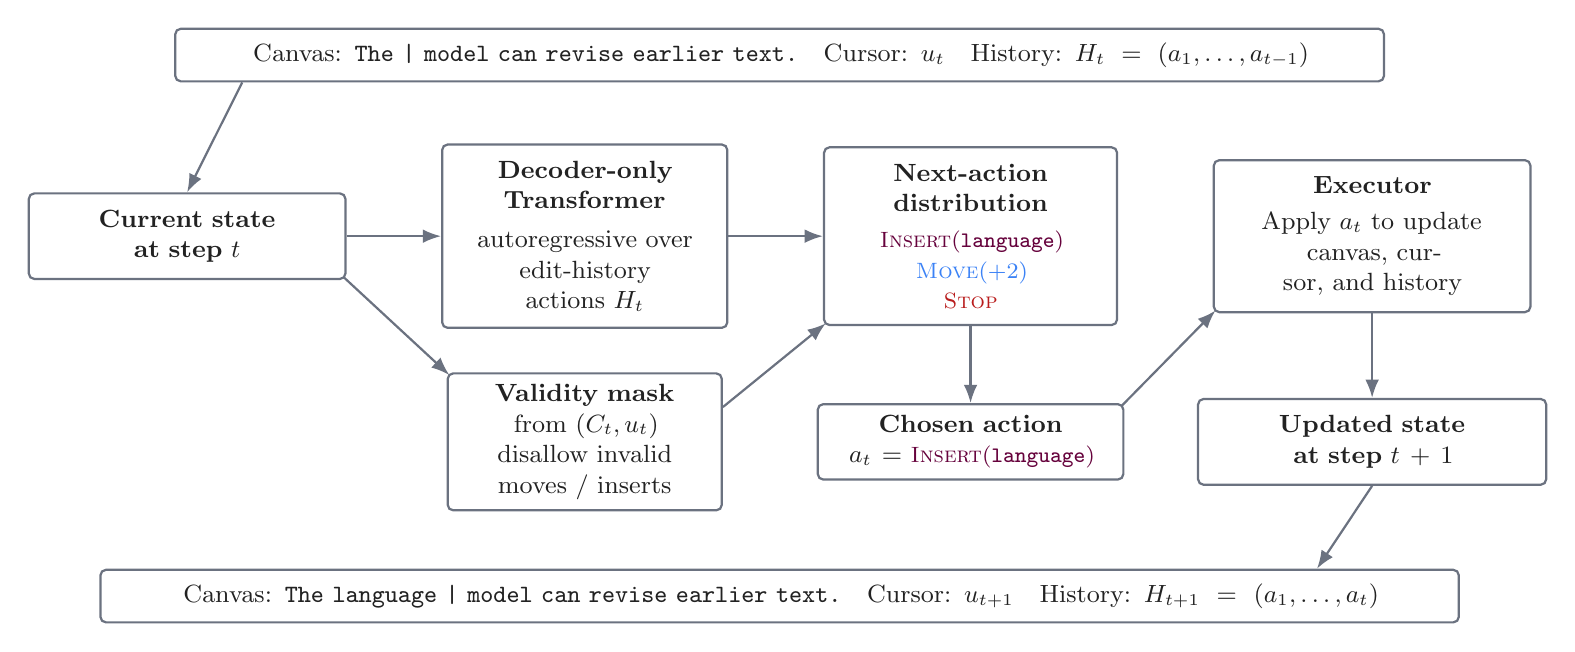
\begin{tikzpicture}[
font=\small,
>=Latex,
box/.style={
draw=FigDarkGray,
rounded corners=2pt,
thick,
fill=white,
inner sep=6pt,
align=center
},
mini/.style={
draw=FigDarkGray,
rounded corners=2pt,
thick,
fill=white,
inner sep=4pt,
align=center
},
arrow/.style={->, thick, draw=FigDarkGray},
every node/.style={text=FigText}
]

% Left state box
\node[box, text width=3.6cm, align=center] (state) {
\textbf{Current state at step $t$}
};

% Transformer box
\node[box, right=1.2cm of state, text width=3.2cm, align=center] (model) {
\textbf{Decoder-only Transformer}\\[3pt]
autoregressive over\\
edit-history actions $H_t$
};

% Mask box
\node[mini, below=0.55cm of model, text width=3.2cm] (mask) {
\textbf{Validity mask} from \textbf{$(C_t,u_t)$}\\
disallow invalid moves / inserts
};

% Action box
\node[box, right=1.2cm of model, text width=3.3cm] (action) {
\textbf{Next-action}\\
\textbf{distribution}\\[2pt]
{\footnotesize\textcolor{FigTyrianPurple}{\textsc{Insert}(\texttt{language})}}\\
{\footnotesize\textcolor{FigBlue}{\textsc{Move}(+2)}}\\
{\footnotesize\textcolor{FigRed}{\textsc{Stop}}}
};

% Chosen action (white bg, only Insert coloured)
\node[mini, fill=white, draw=FigDarkGray, text width=3.6cm] (chosen) at (action |- mask) {
\textbf{Chosen action}\\
$a_t =$ {\footnotesize\textcolor{FigTyrianPurple}{\textsc{Insert}(\texttt{language})}}
};

% Executor
\node[box, right=1.2cm of action, text width=3.6cm] (exec) {
\textbf{Executor}\\[2pt]
Apply $a_t$ to update\\
canvas, cursor, and history
};

% Updated state
\node[box, text width=4.0cm] (updated) at (exec |- mask) {
\textbf{Updated state at step $t+1$}
};

% Horizontal center of the figure content
\coordinate (hcenter) at ($(state.west)!0.5!(exec.east)$);

% Top-wide input block, centered on figure
\node[draw=FigDarkGray, rounded corners=2pt, thick, fill=white, inner sep=5pt,
      anchor=center, text width=15cm, align=center] (input_state)
      at ($(hcenter) + (0, 2.3cm)$) {
Canvas: \texttt{The | model can revise earlier text.}\quad Cursor: $u_t$\quad History: $H_t=(a_1,\dots,a_{t-1})$
};

% Bottom-wide output block, centered on figure
\node[draw=FigDarkGray, rounded corners=2pt, thick, fill=white, inner sep=5pt,
      anchor=center, text width=16.9cm, align=center] (output_state)
      at ($(hcenter |- updated.south) + (0, -1.4cm)$) {
Canvas: \texttt{The language | model can revise earlier text.}\quad Cursor: $u_{t+1}$\quad History: $H_{t+1}=(a_1,\dots,a_t)$
};

% Arrows
\draw[arrow] ($(input_state.south -| state.north) + (0.7cm, 0)$) -- (state.north);
\draw[arrow] (state) -- (model);
\draw[arrow] (model) -- (action);
\draw[arrow] ($(state.south east) + (-1pt, 1pt)$) -- ($(mask.north west) + (1pt, -1pt)$);
\draw[arrow] ($(mask.south east)!0.75!(mask.north east)$) -- ($(action.south west) + (1pt, 1pt)$);
\draw[arrow] (action.south) -- (chosen.north);
\draw[arrow] ($(chosen.north east) + (-1pt, -1pt)$) -- ($(exec.south west) + (1pt, 1pt)$);
\draw[arrow] (exec) -- (updated);
\draw[arrow] (updated.south) -- ($(updated.south |- output_state.north) + (-0.7cm, 0)$);

\end{tikzpicture}%
}% end resizebox
\caption{Reviser decoding at a single step. The model is autoregressive over edit-history actions rather than final text order. At each step it predicts exactly one cursor-relative action, applies a validity mask derived from the current canvas state, and then uses a deterministic executor to update the canvas, cursor, and history.}
\label{fig:reviser_step}
\end{figure}

\subsection{Action Space (Primary Implementation)}
\label{sec:actions}

The action vocabulary is
\[
V_a \;=\; \underbrace{V_c}_{\Insert(\text{token})}\;\cup\;\underbrace{\Mset}_{\Move(\Delta)}\;\cup\;\{\Stop\}.
\]
Here $V_c$ is the normal token vocabulary (each token corresponds to an $\Insert$ action), and $\Mset$ is a small discrete set of move actions (e.g., $\Delta \in \{\pm 1, \pm 2, \pm 4, \dots\}$). $\Stop$ ends generation.

\subsection{Executor: Canvas Update Mathematics}
\label{sec:updates}

Let $C_t = (c_{t,1},\dots,c_{t,\ell_t})$ and cursor $u_t \in \{0,\dots,\ell_t\}$.

For an insertion of token $x \in V_c$ at cursor boundary $u_t \in \{0,\dots,\ell_t\}$,
\[
\Insert(x):\quad
C_{t+1} \;=\;
(c_{t,1}, \dots, c_{t,u_t}, x, c_{t,u_t+1}, \dots, c_{t,\ell_t}),
\qquad
u_{t+1} = u_t + 1.
\]

For a displacement $\Delta \in \mathbb{Z}$ chosen from $\Mset$,
\[
\Move(\Delta):\quad
C_{t+1} = C_t, \qquad
u_{t+1} = u_t + \Delta.
\]
We enforce the post-state constraint $u_{t+1}\in\{0,\dots,\ell_{t+1}\}$ via validity masking (for \Move{}, $\ell_{t+1}=\ell_t$).

\[
\Stop:\quad \text{terminate and output } C_t.
\]

\subsection{Validity Masking}
\label{sec:masking}

At each step, Reviser constructs a valid-action mask based on $(C_t,u_t)$, for example:
\begin{itemize}[leftmargin=*,itemsep=0.2em]
\item forbid moves $\Move(\Delta)$ such that $u_t+\Delta \notin \{0,\dots,\ell_{t+1}\}$ (equivalently $\{0,\dots,\ell_t\}$ for \Move{}),
\item forbid inserting if $\ell_t$ has reached a maximum length,
\item optionally forbid inserting certain reserved tokens.
\end{itemize}
Masking is applied to the action logits before sampling/argmax.

\section{Model}
\label{sec:model}

\subsection{Edit-History Transformer}
\label{sec:history_transformer}

Let $H_t$ be the edit-history action tokens at continuation step $t$. In prefix-seeding decoding, $H_t=(\phA^{\text{pref}}(x),a_1,\dots,a_{t-1})$. We use a single shared embedding table $E \in \mathbb{R}^{|V_a|\times d}$ for all action tokens (including token-valued $\Insert$ actions, $\Move$ actions, and $\Stop$), and a positional embedding table $P^{(H)} \in \mathbb{R}^{T_{\max}\times d}$ for edit-history positions. The history-token embeddings are
\[
e_\tau \;=\; E[a_\tau] + P^{(H)}[\tau], \qquad \tau=1,\dots,t-1.
\]
A standard causal transformer processes $(e_1,\dots,e_{t-1})$ and produces hidden states $(h_1,\dots,h_{t-1})$. The next-action logits are
\[
r_t \;=\; W_{\text{out}}\, h_{t-1} + b_{\text{out}},
\quad
p(a_t \mid H_t, C_t) \;=\; \mathrm{softmax}\!\big(r_t + m_t\big),
\]
where $m_t$ applies the validity mask computed from $(C_t,u_t)$ (invalid actions get $-\infty$). In our experiments, the trunk depends only on $H_t$; the canvas enters through the executed action sequence (which determines what the model has seen) and through masking. Optional designs that add an explicit canvas summary $\mu_t$ (attention pooling) or cross-attention to canvas token representations are described in \Cref{sec:pooling,sec:canvas_cross_attention}.

In the prefix-seeding setting, the prefix $x=(x_1,\dots,x_m)$ enters the model exclusively through the seeded action history: the $m$ prefix-seeding actions $\phA^{\text{pref}}(x) = (\Insert(x_1),\dots,\Insert(x_m))$ occupy the first $m$ positions of $H_t$, so the transformer's self-attention over edit-history tokens directly attends to the full prefix content. No separate encoder or prefix embedding is required; the prefix is fully visible through the standard action-history input stream, and a validity mask applied during continuation decoding prevents the model from editing the prefix region of the canvas.

\subsection{Generation Algorithm}
\label{sec:algo}

\begin{algorithm}[tbp]
\caption{Reviser decoding (insert+move primary implementation)}
\label{alg:reviser_decode}
\begin{algorithmic}[1]
\Require Input prefix $x=(x_1,\dots,x_m)$ (may be empty), max steps $T_{\max}$, max canvas length $L_{\max}$
\State \textbf{Phase 1: Prefix seeding}
\State Initialize canvas $C \leftarrow ()$, cursor $u \leftarrow 0$, history $H \leftarrow ()$
\For{$i = 1,\dots,m$} \State Apply $\Insert(x_i)$: $C \leftarrow (C, x_i)$, $u \leftarrow u+1$, $H \leftarrow (H,\Insert(x_i))$ \EndFor
\State Set $C_1\!\leftarrow\!C$,\; $u_1\!\leftarrow\!m$,\; $H_1\!\leftarrow\!H$ \Comment{$H_1 = \phA^{\text{pref}}(x)$; canvas $= x$; cursor at $m$}
\State \textbf{Phase 2: Continuation decoding}
\For{$t = 1,2,\dots,T_{\max}$}
  \State Compute action logits $r_t \leftarrow f_\theta(H_t)$ \Comment{optionally supply a canvas summary; see Appendix}
  \State Construct validity mask $m_t \leftarrow \textsc{Mask}(C_t,u_t,L_{\max},|x|)$ \Comment{disallow edits to prompt-prefix}
  \State Choose action $a_t \sim \mathrm{softmax}(r_t + m_t)$
  \If{$a_t = \Stop$}
    \State \Return $C_t$
  \Else
    \State Apply executor update $(C_{t+1},u_{t+1}) \leftarrow \textsc{Exec}(C_t,u_t,a_t)$
    \State Append to history $H_{t+1} \leftarrow (H_t, a_t)$
  \EndIf
\EndFor
\State \Return $C_{T_{\max}+1}$ \Comment{fallback if no $\Stop$}
\end{algorithmic}
\end{algorithm}

\Cref{alg:reviser_decode} gives the decoding loop. The loop terminates when $\Stop$ is chosen (or a maximum step budget is reached).
Algorithm~\ref{alg:reviser_decode} has two phases. Phase~1 (prefix-seeding) is deterministic: it replays the prefix as $m$ insert actions, writing $x$ onto the canvas and building $H_1 = \phA^{\text{pref}}(x)$ in the action history. No model call is made during Phase~1. Phase~2 (continuation decoding) is autoregressive: the model conditions on the full seeded history $H_t$ (which begins with $\phA^{\text{pref}}(x)$) and samples continuation actions one at a time. Because the prefix tokens appear as action-history entries, the model's self-attention directly observes prefix content at every continuation step without any additional encoder.

\section{Learning and Training}
\label{sec:training}

\subsection{Worked Example: Edit History Trajectory}
\label{sec:trajectory_example}

This section first shows a sample non-monotonic trajectory in \Cref{fig:trajectory_example}, then gives a separate worked obfuscation--restoration trajectory in \Cref{tab:trajectory}. We render the cursor as a vertical bar ``$|$'' between tokens.

\begin{figure}[t]
\centering
\resizebox{\textwidth}{!}{%
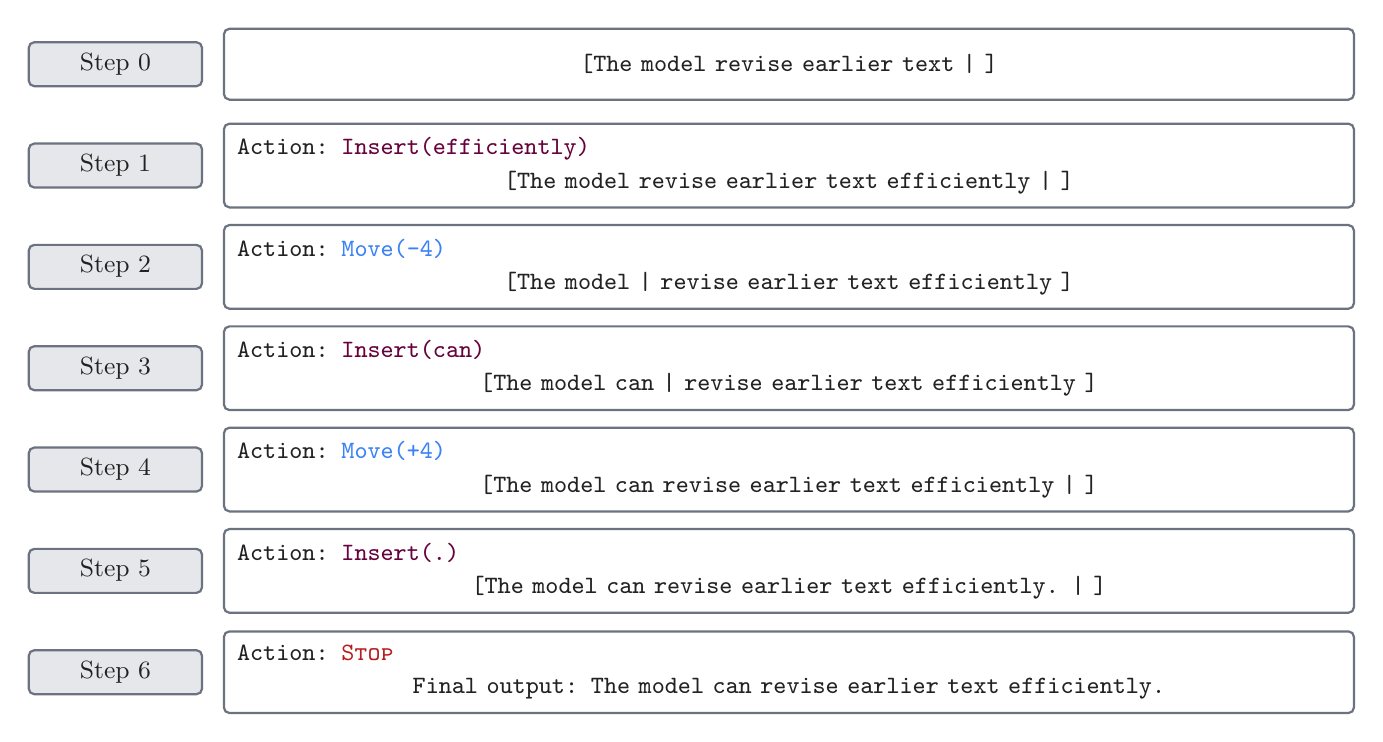
\begin{tikzpicture}[
font=\small,
>=Latex,
rowbox/.style={
draw=FigDarkGray,
rounded corners=2pt,
thick,
fill=white,
inner sep=5pt,
text width=14cm,
minimum height=0.9cm,
anchor=west
},
steplabel/.style={
draw=FigDarkGray,
rounded corners=2pt,
thick,
fill=FigGray,
inner sep=4pt,
minimum width=2.2cm,
align=center
},
every node/.style={text=FigText}
]

% Rows - action left-aligned on top line, canvas centred on lower line
\node[steplabel] (s0) at (0,0) {Step 0};
\node[rowbox, right=0.25cm of s0, align=center] (r0) {%
\texttt{[The model revise earlier text | ]}};

\node[steplabel, below=0.7cm of s0] (s1) {Step 1};
\node[rowbox, right=0.25cm of s1, align=left] (r1) {%
\texttt{Action: \textcolor{FigTyrianPurple}{Insert(efficiently)}}\\[1pt]
\makebox[\linewidth][c]{\texttt{[The model revise earlier text efficiently | ]}}};

\node[steplabel, below=0.7cm of s1] (s2) {Step 2};
\node[rowbox, right=0.25cm of s2, align=left] (r2) {%
\texttt{Action: \textcolor{FigBlue}{Move(-4)}}\\[1pt]
\makebox[\linewidth][c]{\texttt{[The model | revise earlier text efficiently ]}}};

\node[steplabel, below=0.7cm of s2] (s3) {Step 3};
\node[rowbox, right=0.25cm of s3, align=left] (r3) {%
\texttt{Action: \textcolor{FigTyrianPurple}{Insert(can)}}\\[1pt]
\makebox[\linewidth][c]{\texttt{[The model can | revise earlier text efficiently ]}}};

\node[steplabel, below=0.7cm of s3] (s4) {Step 4};
\node[rowbox, right=0.25cm of s4, align=left] (r4) {%
\texttt{Action: \textcolor{FigBlue}{Move(+4)}}\\[1pt]
\makebox[\linewidth][c]{\texttt{[The model can revise earlier text efficiently | ]}}};

\node[steplabel, below=0.7cm of s4] (s5) {Step 5};
\node[rowbox, right=0.25cm of s5, align=left] (r5) {%
\texttt{Action: \textcolor{FigTyrianPurple}{Insert(.)}}\\[1pt]
\makebox[\linewidth][c]{\texttt{[The model can revise earlier text efficiently. | ]}}};

\node[steplabel, below=0.7cm of s5] (s6) {Step 6};
\node[rowbox, right=0.25cm of s6, align=left] (r6) {%
\texttt{Action: \textcolor{FigRed}{\textsc{Stop}}}\\[1pt]
\makebox[\linewidth][c]{\texttt{Final output: The model can revise earlier text efficiently.}}};

\end{tikzpicture}
}% end resizebox
\caption{Illustrative Reviser trajectory. The model need not generate in final left-to-right order: it first appends a word to the end (Step~1), then moves the cursor backward (Step~2), inserts another word into the middle of the canvas (Step~3), returns to the end (Step~4), appends a period (Step~5), and stops (Step~6). This non-monotonic pattern, backward moves followed by mid-canvas insertions, is common in large-scale trajectory statistics, not an edge case.}
\label{fig:trajectory_example}
\end{figure}

\begin{table}[tbp]
\centering
\small
\setlength{\tabcolsep}{6pt}
\begin{tabular}{p{0.47\linewidth}p{0.47\linewidth}}
\toprule
\textbf{Obfuscation (target $\rightarrow$ blank)} &
\textbf{Restoration (blank $\rightarrow$ target)} \\
\midrule
\begin{minipage}[t]{\linewidth}\vspace{0pt}
\begin{enumerate}[leftmargin=*,itemsep=0.2em]
\item Initial\\
\texttt{[Hi,|how are you?]}

\item $\Delete$\\
\texttt{[Hi|how are you?]}

\item $\Delete$\\
\texttt{[|how are you?]}

\item $\Move(+4)$\\
\texttt{[how are you?|]}

\item $\Delete$\\
\texttt{[how are you|]}

\item $\Delete$\\
\texttt{[how are|]}

\item $\Delete$\\
\texttt{[how|]}

\item $\Delete$\\
\texttt{[|]}
\end{enumerate}
\end{minipage}
&
\begin{minipage}[t]{\linewidth}\vspace{0pt}
\begin{enumerate}[leftmargin=*,itemsep=0.2em]
\item Initial\\
\texttt{[|]}

\item $\Insert$(\texttt{how})\\
\texttt{[how|]}

\item $\Insert$(\texttt{are})\\
\texttt{[how are|]}

\item $\Insert$(\texttt{you})\\
\texttt{[how are you|]}

\item $\Insert$(\texttt{?})\\
\texttt{[how are you?|]}

\item $\Move(-4)$\\
\texttt{[|how are you?]}

\item $\Insert$(\texttt{Hi})\\
\texttt{[Hi|how are you?]}

\item $\Insert$(\texttt{,})\\
\texttt{[Hi,|how are you?]}

\item $\Stop$\\
\texttt{[Hi,|how are you?]}
\end{enumerate}
\end{minipage}
\\
\bottomrule
\end{tabular}
\caption{Side-by-side obfuscation and restoration trajectory for a full continuation without a prefix.}
\label{tab:trajectory}
\end{table}

Reviser is trained to predict the next action token under teacher forcing on action trajectories. Training follows the same two-phase structure as decoding: a deterministic prefix-seeding phase $\phA^{\text{pref}}(x)$ seeds the canvas and action history, followed by a learned restoration phase $\phA^{\text{rest}}(y)$ over the continuation target; NLL is computed only over $\phA^{\text{rest}}(y)$. Given a restoration trajectory $\phA^{\text{rest}} = (a_1, \dots, a_T)$, we minimize the standard negative log-likelihood:
\[
\mathcal{L}(\theta) \;=\; -\sum_{t=1}^{T} \log p_\theta(a_t \mid s_t).
\]

\subsection{Obfuscation--Restoration Supervision (Main Training Procedure)}
\label{sec:obf_restoration}

\begin{algorithm}[t]
\caption{Obfuscation--restoration trajectory generation (primary implementation)}
\label{alg:obf_restore}
\begin{algorithmic}[1]
\Require Target tokens $y=(y_1,\dots,y_n)$, move set $\Mset$, max steps $K_{\max}$
\State Initialize canvas $C \leftarrow y$; initialize cursor $u \leftarrow \textsc{Uniform}(\{0,\dots,n\})$
\State Initialize empty obfuscation action list $B \leftarrow ()$ and empty metadata list $\mathcal{D}\leftarrow()$
\For{$k=1,2,\dots,K_{\max}$}
\If{$|C| = 0$} \textbf{break} \EndIf
\State Sample an obfuscation action $b_k \sim \pi_{\text{obf}}(\cdot \mid C,u)$ from \textsc{Delete} or a move action \Move($\Delta$), using validity masking
\If{$b_k = \Delete$}
\State Let $x \leftarrow c_{u}$ be the token immediately left of the cursor boundary
\State Delete $x$ from $C$ and update cursor $u \leftarrow u-1$
\State Append $x$ to $\mathcal{D}$
\Else
\State Apply cursor move $u \leftarrow u+\Delta$
\EndIf
\State Append $b_k$ to $B$
\EndFor
\State Let $n_{\text{obf}} \leftarrow |B|$
\State Construct restoration actions $\phA\leftarrow()$ by iterating $B$ from last to first:
\State Treat $\mathcal{D}$ as a LIFO stack for deleted-token replay
\For{$k=n_{\text{obf}},n_{\text{obf}}-1,\dots,1$}
\If{$b_k=\textsc{Delete}$} \State pop $x$ from $\mathcal{D}$ and append $\Insert(x)$ to $\phA$
\Else \State append $\Move(-\Delta)$ to $\phA$
\EndIf
\EndFor
\State Append $\Stop$ to $\phA$; \Return obfuscated start state and restoration trajectory $\phA$
\end{algorithmic}
\end{algorithm}

\Cref{alg:obf_restore} specifies the offline trajectory-construction procedure used for supervision. It samples an obfuscation sequence over the continuation canvas, records deleted tokens, and then builds the restoration sequence by reversing and inverting the obfuscation actions, finally appending $\Stop$.

We construct training data using paired trajectories (see \Cref{tab:trajectory} for a concrete side-by-side example):
(i) an obfuscation trajectory that transforms a target sequence into a blank canvas state, and
(ii) a restoration trajectory $\phA^{\text{rest}}(y)$ that transforms the blank state back to the target.
The full supervised sequence for a document split into prefix $x$ and continuation target $y$ is
\[
\phA \;=\; \bigl(\phA^{\text{pref}}(x),\; \phA^{\text{rest}}(y)\bigr),
\]
where $\phA^{\text{pref}}(x) = (\Insert(x_1),\dots,\Insert(x_m))$ is the deterministic prefix-seeding phase and $\phA^{\text{rest}}(y)$ is the restoration trajectory over the continuation target $y=(y_1,\dots,y_n)$. In richer action spaces that include temporary obfuscation-only insertions later removed by restoration deletes, those transient insertions are excluded from the loss because they are often random/noise tokens introduced only to create states that include delete actions, not meaningful target-response content. In our primary experiments (insert+move+$\Stop$ action set at training and test time), obfuscation/restoration is applied only to $y$ (the prompt prefix $x$ is not edited), and we construct obfuscations using only deletions and moves, with restoration defined as the inverse mapping (each obfuscation deletion becomes an insertion of the deleted token, and each obfuscation move becomes the opposite move).

We generate an obfuscation trajectory by initializing the editable canvas to the continuation target and inserting the cursor at a uniformly random editable boundary, i.e., $C \leftarrow y$ and $u \sim \mathrm{Uniform}(\{0,\dots,|y|\})$. At each obfuscation step, we sample an action from a simple state-dependent random policy with validity masking: with probability $0.8$ we apply \textsc{Delete}, which deletes the token immediately to the left of the cursor; with probability $0.2$ we apply a move action \textsc{Move}($\Delta$), where $\Delta$ is sampled uniformly from the set of valid moves (i.e., those satisfying $u+\Delta\in\{0,\dots,\ell\}$). We store the resulting obfuscation action sequence as $B=(b_1,\dots,b_{n_{\text{obf}}})$, where $n_{\text{obf}}$ is the number of obfuscation steps until termination. For each deletion step, we additionally record the identity of the deleted token in temporal order in an aligned side list $\mathcal{D}=(d_1,\dots,d_{n_{\text{del}}})$, where $n_{\text{del}}$ is the number of deletions in $B$.

We represent cursor moves using a finite discrete set of displacements $\Mset$. In our implementation we use powers-of-two jumps up to a maximum displacement:
\[
\Mset \;=\; \{\, \pm 2^k \mid k\in\mathbb{Z}_{\ge 0},\; 2^k \le \text{max\_move}\,\}.
\]
At each step, we form the state-dependent valid subset $\Mset(C_t,u_t) = \{\Delta\in\Mset : u_t+\Delta\in\{0,\dots,\ell_t\}\}$ and sample $\Delta$ uniformly from $\Mset(C_t,u_t)$.

We terminate obfuscation when the editable canvas is empty (i.e., $\ell=0$, leaving only the cursor boundary). If an obfuscation trajectory fails to reach $\ell=0$ within a maximum step budget $K_{\max}$, we discard the sample and resample a new trajectory.

Given an obfuscation trajectory $B=(b_1,\dots,b_{n_{\text{obf}}})$ and deleted-token metadata $\mathcal{D}=(d_1,\dots,d_{n_{\text{del}}})$, we construct a restoration trajectory $\phA=(a_1,\dots,a_T)$ by scanning $B$ from last to first and replacing each obfuscation action with its inverse restoration action. We treat $\mathcal{D}$ as a stack in temporal order and, whenever the reversed scan encounters a \textsc{Delete}, we pop the most recently deleted token from $\mathcal{D}$ (LIFO order). For each $k=n_{\text{obf}},n_{\text{obf}}-1,\dots,1$, we emit a restoration action
\[
a \;\leftarrow\;
\begin{cases}
\Insert(x) \text{ where } x=\mathrm{pop}(\mathcal{D}) & \text{if } b_k=\textsc{Delete},\\
\textsc{Move}(-\Delta) & \text{if } b_k=\textsc{Move}(\Delta),
\end{cases}
\]
and append these emitted actions in the scan order to form $\phA$. Finally, we append $\Stop$ after the last restorative edit. In this strict-inverse construction, we produce one restoration action per obfuscation action, hence $T_{\text{rest}}=n_{\text{obf}}+1$. Executing $\phA$ from a blank canvas state deterministically reconstructs the target sequence and cursor position.

This reverse-inverse construction is a simple but effective supervision source. Reversing the obfuscation trajectory yields restoration actions that are guaranteed to be state-consistent with the executor dynamics, so each training target is a valid next edit for the current canvas/cursor state rather than a synthetic label detached from state. In practice, this generates dense edit-history data that teaches the model to repair a corrupted canvas into a coherent sequence using the same action interface used at inference, which we find produces strong generation quality and robust non-monotonic editing behavior.

Instead of strict inverse mapping, restoration trajectories can be constructed by (i) an oracle policy, (ii) alignment/diff procedures, (iii) dynamic programming, or (iv) constrained search; and one can also use human text-edit traces, aggregate trajectories under the learned policy (DAgger), or fine-tune with RL. We discuss these variants in the Appendix (\Cref{sec:dagger,sec:rl}).

Because the model's actions affect future states, naive supervised learning can suffer from compounding error. We consider two standard remedies: (i) dataset aggregation (DAgger-style), where we roll out the learned policy and label visited states with an oracle action \citep{ross2011dagger}, and (ii) reinforcement learning fine-tuning (e.g., PPO-style), where rewards are defined over completed trajectories \citep{schulman2017ppo}. In the reported experiments, we use supervised learning only (teacher forcing on restoration trajectories), without DAgger or RL fine-tuning (see Appendix~\Cref{sec:dagger,sec:rl}).

\paragraph{Limitations of synthetic restoration trajectories.}
Our training data is constructed by applying random obfuscation trajectories and training the model to invert them. While this provides a simple and scalable source of supervision, these trajectories do not reflect the structure of humanlike editing behavior. In particular, human edits are typically purposeful and context-dependent, involving targeted insertions, deletions, and refinements rather than random perturbations. As a result, the learned editing policies may differ from those that would arise from training on naturally occurring edit sequences. We expect that training on datasets of real edits, such as document revision histories or code editing traces, could yield more efficient and semantically meaningful editing strategies.

\section{Experiments}
\label{sec:experiments}

\subsection{Setup}
\label{sec:setup_exp}

We evaluate Reviser on a C4 continuation benchmark built from the English validation split of \texttt{allenai/c4}, comparing against autoregressive baselines at matched scales and non-autoregressive diffusion baselines. We pre-filter examples to total GPT-2 token length 144 to 216, use a 35-token prefix, and evaluate continuation quality toward a 180-token total sequence target.

We report results for two Reviser checkpoints: 100M and 300M. For the SEDD/MDLM comparison, we evaluate three seeds (\texttt{123}, \texttt{124}, \texttt{125}) with 1000 prompts per seed (3000 total per model). All main-text results use decoding with a maximum of 256 actions.
For the diffusion baselines, both SEDD and MDLM are decoded with 128 diffusion steps.
For models we train ourselves, we use matched 30B-token budgets: the trained AR baselines are trained on 30B text tokens, and Reviser models are trained on 30B edit-history tokens (including \Move{} tokens). Because about 20\% of Reviser training actions are \Move{} actions, Reviser is exposed to fewer word tokens than the AR models under this matched token-budget accounting.

We report two metric families. First, we run pairwise 1v1 with-input arenas where the judge sees the prompt and both candidate continuations and selects a winner. For each arena example, we randomize candidate order (which model is shown as A vs.\ B) before constructing the judge input. We use Skywork-Critic-8B \citep{skywork2024critic} as the judge throughout all arena comparisons. Second, evalPPL is computed on continuation tokens (lower is better), using two evaluator backbones: an autoregressive evaluator (GPT-2 Large) and a diffusion-style evaluator (Dream-7B). Reporting both reduces evaluator-family bias for Reviser's nonstandard edit-action generation interface. We do not report regular teacher-forced PPL over Reviser action sequences because restoration trajectories are randomized and non-unique for a given final continuation, so trajectory-level likelihood is not a canonical, directly comparable quantity. Unless otherwise noted, all benchmark and arena results in this section are computed on 3000 samples.
For reproducibility, code/configs/results are available at \texttt{https://github.com/Sean-Diab/Reviser}, and released Reviser checkpoints are available at \texttt{https://huggingface.co/sean-diab/reviser-checkpoints}.

\subsection{Reviser vs.\ AR Baseline (100M and 300M)}
\label{sec:ar_baseline_matched}

We compare Reviser against autoregressive transformers of identical architecture trained on FineWeb data (the same distribution used to train Reviser) at both 100M and 300M scales. Throughout this section, we refer to these models as the AR baseline at each scale. This is a challenging setting: the AR model is on its home data and optimises the exact objective that evalPPL measures. Results are shown in \Cref{tab:arena_vs_ar_baseline}. The judge prefers Reviser at both scales: \num{61.3}\% vs.\ \num{38.7}\% at 100M, and \num{54.4}\% vs.\ \num{45.6}\% at 300M.

\begin{table}[tbp]
\centering
\small
\setlength{\tabcolsep}{5pt}
\begin{tabular}{lcc}
\toprule
AR Baseline & Reviser WR $\uparrow$ & AR WR $\uparrow$ \\
\midrule
AR Baseline 100M & \num{61.3}\% & \num{38.7}\% \\
AR Baseline 300M & \num{54.4}\% & \num{45.6}\% \\
\bottomrule
\end{tabular}
\caption{Reviser vs.\ AR baseline at 100M and 300M: arena win rates.}
\label{tab:arena_vs_ar_baseline}
\end{table}

\begin{table}[tbp]
\centering
\small
\setlength{\tabcolsep}{7pt}
\begin{tabular}{lcc}
\toprule
Model & evalPPL GPT-2 Large $\downarrow$ & evalPPL Dream 7B $\downarrow$ \\
\midrule
AR Baseline 100M & \num{13.5210} & \num{13.9584} \\
Reviser 100M & \num{30.6355} & \num{22.6693} \\
AR Baseline 300M & \num{12.5122} & \num{12.0203} \\
Reviser 300M & \num{17.7700} & \num{15.7733} \\
\bottomrule
\end{tabular}
\caption{Reviser vs.\ AR baseline at 100M and 300M: evalPPL results (C4 decoding). Lower is better.}
\label{tab:evalppl_vs_ar_baseline}
\end{table}

Although Reviser has higher evalPPL than the AR baseline in \Cref{tab:evalppl_vs_ar_baseline}, its arena results remain strong (\Cref{tab:arena_vs_ar_baseline}). A likely reason is metric mismatch across generation paradigms: evalPPL is computed with an autoregressive scorer, while Reviser decodes via edit actions. The very high evalPPL values observed for SEDD/MDLM in \Cref{tab:evalppl_vs_diffusion} are consistent with this effect.

\subsection{Reviser vs.\ AR Baselines}
\label{sec:ar_baselines}

We evaluate Reviser in direct 1v1 arena matchups against a range of publicly available autoregressive models at roughly size-matched scales.
All pairwise arena matchups in this subsection use 3000 samples per comparison.

\begin{table}[tbp]
\centering
\small
\setlength{\tabcolsep}{5pt}
\begin{tabular}{l ccc ccc}
\toprule
Model & 100M Size & Rev WR $\uparrow$ & AR WR $\uparrow$ & 300M Size & Rev WR $\uparrow$ & AR WR $\uparrow$ \\
\midrule
Cerebras                & 111M & \num{72.1}\% & \num{27.9}\% & 256M & \num{71.3}\% & \num{28.7}\% \\
Pythia                  & 160M & \num{68.8}\% & \num{31.2}\% & 410M & \num{51.3}\% & \num{48.7}\% \\
GPT-2                   & 117M & \num{58.6}\% & \num{41.4}\% & 345M & \num{50.4}\% & \num{49.6}\% \\
OPT                     & 125M & \num{53.9}\% & \num{46.1}\% & 350M & \num{49.9}\% & \num{50.1}\% \\
\bottomrule
\end{tabular}
\caption{Reviser vs.\ AR baselines at 100M and 300M scales: arena win rates under Skywork-Critic-8B.}
\label{tab:ar_baselines_100m}
\end{table}

At 100M scale, Reviser is preferred to all four AR baselines in this comparison, with especially large margins against Cerebras-GPT-111M and Pythia-160M. At 300M scale, Reviser remains competitive: it strongly outperforms Cerebras-GPT-256M and is approximately tied with Pythia-410M, GPT-2 Medium, and OPT-350M. Overall, these AR comparisons indicate a robust and promising profile.

\subsection{Results: Reviser vs.\ SEDD and MDLM}
\label{sec:results}

\Cref{tab:arena_vs_diffusion} reports arena win rates against both diffusion baselines and shows that Reviser wins all three matchups, with its largest margin against SEDD Small 169M (\num{85.93}\% vs.\ \num{14.07}\%), followed by MDLM 170M (\num{78.33}\% vs.\ \num{21.67}\%), and SEDD Absorb 353M (\num{68.47}\% vs.\ \num{31.53}\%). \Cref{tab:evalppl_vs_diffusion} reports the corresponding evalPPL values and shows the same qualitative pattern: Reviser is much lower than SEDD/MDLM under both evaluators at both available scales. MDLM does not have a comparable 300M checkpoint in our setup, so we omit MDLM-300M comparisons.

\begin{table}[tbp]
\centering
\small
\setlength{\tabcolsep}{5pt}
\begin{tabular}{lccc}
\toprule
Comparison & Reviser WR $\uparrow$ & Baseline WR $\uparrow$ \\
\midrule
SEDD Small 169M  & \num{85.93}\% & \num{14.07}\% \\
SEDD Absorb 353M & \num{68.47}\% & \num{31.53}\% \\
MDLM 170M        & \num{78.33}\% & \num{21.67}\% \\
\bottomrule
\end{tabular}
\caption{Reviser vs.\ SEDD and MDLM: arena win rates.}
\label{tab:arena_vs_diffusion}
\end{table}

\begin{table}[tbp]
\centering
\small
\setlength{\tabcolsep}{7pt}
\begin{tabular}{lcc}
\toprule
Model & evalPPL GPT-2 Large $\downarrow$ & evalPPL Dream 7B $\downarrow$ \\
\midrule
Reviser 100M & \num{30.6355} & \num{22.6693} \\
SEDD Small 169M & \num{158.7165} & \num{117.0477} \\
MDLM 170M & \num{144.6948} & \num{94.3026} \\
\midrule
Reviser 300M & \num{17.7700} & \num{15.7733} \\
SEDD Absorb 353M & \num{98.6821} & \num{83.2764} \\
\bottomrule
\end{tabular}
\caption{Reviser vs.\ SEDD and MDLM: evalPPL results (C4 decoding). Lower is better. MDLM 300M is omitted because no comparable checkpoint is available in this setup.}
\label{tab:evalppl_vs_diffusion}
\end{table}

\subsection{MAUVE}
\label{sec:mauve}

We also report MAUVE under a shared-3k protocol (\Cref{tab:mauve_all}): 3000 shared C4 examples, with references and model outputs truncated to 100 tokens, and BERT pseudo-loglikelihood features used for MAUVE computation. MAUVE measures distributional overlap between model outputs and references, with higher values indicating closer distributional match.

\begin{table}[tbp]
\centering
\small
\setlength{\tabcolsep}{7pt}
\begin{tabular}{lc}
\toprule
Model & MAUVE $\uparrow$ \\
\midrule
AR Baseline 100M & \num{0.9038} \\
AR Baseline 300M & \num{0.9103} \\
\midrule
Reviser 300M & \num{0.9349} \\
GPT-2 117M & \num{0.8770} \\
GPT-2 Medium 345M & \num{0.8230} \\
Reviser 100M & \num{0.8392} \\
\midrule
SEDD Absorb 353M & \num{0.3594} \\
SEDD Small 169M & \num{0.1798} \\
MDLM 170M & \num{0.1509} \\
\bottomrule
\end{tabular}
\caption{Combined MAUVE results on the shared 3000-example C4 subset, using BERT pseudo-loglikelihood features and 100-token truncation for both references and model outputs. Higher is better.}
\label{tab:mauve_all}
\end{table}

\Cref{tab:mauve_all} shows that Reviser 300M achieves the strongest MAUVE in this comparison, while diffusion baselines (SEDD/MDLM) are substantially lower, consistent with the arena and evalPPL trends.

\subsection{Trajectory Statistics}
\label{sec:trajectory_stats}

\Cref{tab:trajectory_stats} shows that Reviser uses the edit interface in a strongly non-AR way. Move actions are frequent, backward moves dominate, and almost all insertions are non-end (mid-canvas) insertions. In every evaluated example, the trajectory contains at least one backward revision event, confirming that the model is not merely emulating a pure end-append decoder.

\begin{table}[tbp]
\centering
\small
\setlength{\tabcolsep}{6pt}
\begin{tabular}{lcc}
\toprule
Statistic (averaged across seeds) & 100M & 300M \\
\midrule
Actions per output token & \num{1.51} & \num{1.40} \\
Insert fraction & 67\% & 72\% \\
Move fraction & 33\% & 28\% \\
Mean $|\Delta|$ move distance & \num{4.92} & \num{6.05} \\
Move-distance mass on 1/2/4/8 moves (\%) & 40.5, 23.3, 15.8, 10.0 & 37.4, 22.7, 15.5, 11.1 \\
Fraction backward moves & \num{65.5}\% & \num{64.5}\% \\
Mean insertion relative position & \num{0.41} & \num{0.42} \\
Fraction end-appends (cursor at end) & \num{3.9}\% & \num{3.1}\% \\
Fraction non end-appends & \num{96.1}\% & \num{96.9}\% \\
Examples with $\geq 1$ backward revision & 100\% & 100\% \\
\bottomrule
\end{tabular}
\caption{Reviser trajectory diagnostics in decoding. ``Backward revision'' means at least one backward move followed by subsequent insertion into an earlier canvas region.}
\label{tab:trajectory_stats}
\end{table}
\section{Limitations}
\label{sec:limitations}
Reviser is sequential in action space, so decoding is not fully parallelizable over final-token positions. As a result, throughput is still constrained by step-by-step generation, even though the model can revise non-monotonically.

Quality also depends on the supervision trajectories. Because training is based on synthetic obfuscation--restoration paths, performance can degrade under distribution shift and may exhibit compounding error when the model visits states that are weakly represented in training data.

The primary insert+move action set supports flexible revision, but some edits may require longer trajectories than richer operators (e.g., delete/replace). In addition, the history-only trunk must maintain an implicit representation of the current canvas from the edit-history stream. In our reported runs, we did not observe this as a practical bottleneck, even for long trajectories, which is consistent with model capacity at 100M/300M. If needed, explicit state-conditioning mechanisms such as pooled canvas embeddings or cross-attention to canvas representations (\Cref{sec:pooling,sec:canvas_cross_attention}) provide direct mitigation.

\section{Future Work}
\label{sec:future}
The current results suggest several clear directions for improving Reviser. The main opportunities are to expand the action space beyond insert+move, strengthen state conditioning beyond the current history-only trunk, and move beyond fixed synthetic restoration trajectories toward training procedures that better reflect the model's own inference-time distribution. More broadly, we view the present system as a proof of concept for autoregression over edit actions, and expect future variants to improve both output quality and editing efficiency while preserving the lightweight one-action decoding interface.

\paragraph{Learning beyond supervised trajectories.}
While we train Reviser using supervised restoration trajectories, an important next step is to move from synthetic trajectories to real edit supervision, e.g., human editing traces where people iteratively revise drafts, document revision histories, or code editing logs. The action-based interface is also compatible with more flexible training paradigms such as reinforcement learning or dataset aggregation (DAgger; see Appendix~\Cref{sec:dagger,sec:rl}). In principle, any editing idea that can be represented as a token (or short token sequence) can be emitted by the transformer as an executable edit action, opening a broad and creative design space for richer supervision and editing behavior. Together, these approaches could allow the model to learn editing strategies under its own distribution, rather than following fixed trajectories. We leave empirical investigation of these directions to future work.

\paragraph{Flexible generation order as a potential advantage.}
A key property of Reviser is that it can build outputs in whatever order is useful for the task, rather than being constrained to final left-to-right token order. This gives the model an explicit draft-and-revise mechanism during generation: it can insert provisional content, move backward, and refine earlier regions before stopping. We hypothesize that, if learned reliably at scale, this flexibility may provide a meaningful quality advantage over strictly AR decoding, particularly in settings where iterative revision is important.

\paragraph{Structured editing and agent-based applications.}
Beyond text continuation, the cursor-action formulation also suggests applications to structured editing tasks such as code or document modification. Modern agent systems typically edit files by proposing diffs or patches over whole sequences \citep{yang2024sweagent,gauthier2024aider}; this can be inference-inefficient, since the model must spend tokens to emit a diff/patch command rather than directly editing the target content. In contrast, Reviser operates through localized cursor actions on a mutable canvas, which may provide a more direct interface for incremental editing. In such settings, richer edit operators such as \Delete, \Replace, or span-level edits would likely make editing substantially more efficient by allowing the model to modify existing content directly rather than simulating corrections through longer insert-and-move trajectories. This structural alignment suggests the potential for more efficient editing workflows.

\section{Conclusion}
\label{sec:conclusion}
Reviser shows that a simple autoregressive-over-edits decoder, seeded with a deterministic prefix-seeding history and then decoding continuations via cursor actions, can produce genuinely non-monotonic text generation with a lightweight next-action interface. Across our experiments, the model performs frequent backward moves and mid-canvas insertions, is strongly preferred to the diffusion baselines we tested, and is competitive with roughly size-matched AR baselines. Overall, these results provide a strong example that edit-history autoregression is a practical and scalable path to models that can actively revise and improve their responses during generation.

\bibliographystyle{abbrvnat}
\bibliography{references}

\appendix

\tableofcontents
\section{Additional Reviser Variants}

\subsection{Other Edit Operators}
\label{sec:optional_ops}
This appendix subsection lists additional edit operators that can be supported by the same deterministic executor and validity masking used for \Insert/\Move/\Stop.
More generally, any editing idea that can be represented by a token can be implemented as an action token (or a short composition of action tokens) and emitted by the transformer, provided the executor semantics are defined and validity-masked.

Replace the token immediately to the left of the cursor boundary with a new token $x\in V_A$:
\[
\Replace(x):\quad
C_{t+1} \;=\;
(c_{t,1},\dots,c_{t,u_t-1},x,c_{t,u_t+1},\dots,c_{t,\ell_t}),
\qquad
u_{t+1}=u_t.
\]
Validity constraint: $u_t\in\{1,\dots,\ell_t\}$. (Equivalently, \Replace$(x)$ can be viewed as $\Delete$ followed by \Insert$(x)$ at boundary $u_t-1$, but we include it as a single macro-action.)

For a span length $k\in\{1,\dots,u_t\}$, delete the last $k$ tokens immediately to the left of the cursor boundary:
\[
\SpanDelete(k):\quad
C_{t+1} \;=\;
(c_{t,1},\dots,c_{t,u_t-k},c_{t,u_t+1},\dots,c_{t,\ell_t}),
\qquad
u_{t+1}=u_t-k.
\]
Validity constraint: $1\le k \le u_t$.

Swap the last two tokens immediately to the left of the cursor boundary:
\[
\Swap:\quad
C_{t+1} \;=\;
(c_{t,1},\dots,c_{t,u_t-2},c_{t,u_t},c_{t,u_t-1},c_{t,u_t+1},\dots,c_{t,\ell_t}),
\qquad
u_{t+1}=u_t.
\]
Validity constraint: $u_t\in\{2,\dots,\ell_t\}$.

Move a contiguous span of length $k$ that ends at the token immediately left of the cursor boundary (i.e., indices $u_t-k+1,\dots,u_t$) to a destination boundary $j$ in the pre-removal canvas:
\[
\SpanMove(k,j):\quad
C_{t+1}=
\]
\[
\begin{cases}
(\underbrace{c_{t,1},\dots,c_{t,j}}_{\text{left context}},\;
\underbrace{c_{t,u_t-k+1},\dots,c_{t,u_t}}_{\text{moved span}},\;
\underbrace{c_{t,j+1},\dots,c_{t,u_t-k}}_{\text{boosted context}},\;
\underbrace{c_{t,u_t+1},\dots,c_{t,\ell_t}}_{\text{right context}}),
& \text{if } 1\le j\le u_t-k,\\[1mm]
(\underbrace{c_{t,1},\dots,c_{t,u_t-k}}_{\text{left context}},\;
\underbrace{c_{t,u_t+1},\dots,c_{t,j}}_{\text{collapsed context}},\;
\underbrace{c_{t,u_t-k+1},\dots,c_{t,u_t}}_{\text{moved span}},\;
\underbrace{c_{t,j+1},\dots,c_{t,\ell_t}}_{\text{right context}}),
& \text{if } u_t\le j\le \ell_t.
\end{cases}
\]
\[
u_{t+1}=
\begin{cases}
u_t, & \text{if } 1\le j\le u_t-k,\\
j,   & \text{if } u_t\le j\le \ell_t.
\end{cases}
\]
Validity constraints: $1\le k\le u_t$ and $j\in\{1,\dots,u_t-k\}\cup\{u_t,\dots,\ell_t\}$ (enforced by masking). Underbraced segments may be empty.

Copy (without removing) the length-$k$ span immediately left of the cursor boundary and insert it at boundary $j\in\{0,\dots,\ell_t\}$:
\[
\SpanCopy(k,j):\quad
C_{t+1} \;=\;
(\underbrace{c_{t,1},\dots,c_{t,j}}_{\text{left context}},\;
\underbrace{c_{t,u_t-k+1},\dots,c_{t,u_t}}_{\text{copied context}},\;
\underbrace{c_{t,j+1},\dots,c_{t,\ell_t}}_{\text{right context}}),
\qquad
u_{t+1}=j+k,
\]
with validity constraint $1\le k\le u_t$.
For both \SpanCopy{} and \SpanMove{}, one can analogously copy/move spans taken from the right side of the cursor; we omit that symmetric math here.

All of the operators above admit straightforward supervised training using obfuscation restoration trajectories. The key observation is that each edit operator has a natural inverse. When temporary obfuscation-only insertions are used and later deleted, those transient insertions are treated as latent noise and excluded from the training loss because they are often random artifacts rather than meaningful target-response content.\\


\subsection{Conditioning on the Canvas Representations via Pooled Canvas Embeddings}
\label{sec:pooling}

This subsection describes a variant in which action selection uses an explicit pooled summary of the current canvas. The motivation is simple: in a history-only trunk, canvas content is visible only indirectly through past actions and masking; adding a pooled canvas summary provides a direct channel for the model to ``see'' the current canvas state when choosing the next action. Our reported experiments use a history-only trunk without this module.

Attention pooling is just one instantiation of a broader idea: collapse variable-length canvas information into a fixed-size per-step vector (or small set of vectors) that can condition next-action prediction. There are many ways to perform this collapse (e.g., learned pooling queries, mean/max pooling with projections, convolutional pooling, recurrent summarizers, sparse/selective pooling, or learned routers). We use attention pooling here as a simple reference design.

Embed canvas tokens with the same shared token embedding table $E$ as action tokens and a dedicated canvas positional table $P^{(C)}$. For the current canvas $C_t=(c_{t,1},\dots,c_{t,\ell_t})$, define
\[
z_i \;=\; E[c_{t,i}] + P^{(C)}[i], \qquad i=1,\dots,\ell_t.
\]
Let $q \in \mathbb{R}^{d}$ be a learned query vector. Compute attention weights:
\[
s_i \;=\; q^\top z_i, \qquad
\alpha_i \;=\; \frac{\exp(s_i)}{\sum_{j=1}^{\ell_t}\exp(s_j)}.
\]
The pooled canvas embedding is:
\[
\mu_t \;=\; \sum_{i=1}^{\ell_t} \alpha_i z_i \;\in\; \mathbb{R}^{d}.
\]

In this variant, one injects the pooled canvas summary as an additive conditioning term on history-token inputs:
\[
x_\tau \;=\; e_\tau \;+\; \mu_t, \quad \tau=1,\dots,t-1.
\]
One may instead apply a learned linear projection $W_m \in \mathbb{R}^{d\times d}$:
\[
x_\tau \;=\; e_\tau \;+\; W_m\, \mu_t,
\]
including the identity (no projection) as the simplest choice.

\subsection{Cross-Attention to Canvas Representations}
\label{sec:canvas_cross_attention}

Another optional design lets the history stream cross-attend to the full canvas sequence (often paired with or used instead of a single pooled canvas vector; \Cref{sec:pooling}). Let $H_t \in \mathbb{R}^{m\times d}$ denote the history-stream hidden states at step $t$ (the model's input token stream), and let $\mu_t\in\mathbb{R}^d$ be the pooled canvas embedding from \Cref{sec:pooling}. Define $\mathbf{M}_t \in \mathbb{R}^{n\times d}$ as the pooled-canvas matrix whose rows are all equal to $\mu_t^\top$. In a cross-attention block, we compute queries from the history and keys/values from this pooled-canvas matrix:
\[
Q_t = H_t W_Q,\qquad K_t = \mathbf{M}_t W_K,\qquad V_t = \mathbf{M}_t W_V,
\]
and add the resulting cross-attention output as a residual update:
\[
\widetilde{H}_t
= H_t + \textsc{Softmax}\!\Big(\frac{Q_tK_t^\top}{\sqrt{d_k}} + M\Big)V_t.
\]


In our main implementation, cross-attention is inserted after the history self-attention (and before the MLP) in each transformer layer, though in practice it often suffices to apply it only in the last $L_{\text{ca}}$ layers to reduce cost. The cross-attention update can also be gated:

\[
\widetilde{H}_t = H_t + \lambda_{\text{ca}}\cdot \textsc{Softmax}\!\Big(\frac{Q_tK_t^\top}{\sqrt{d_k}} + M\Big)V_t,
\]
with either a learned scalar $\lambda_{\text{ca}}$ per layer or a small gating MLP.
With this pooled-canvas matrix, the block uses a compressed canvas memory derived from $\mu_t$ rather than per-token canvas states; in practice one can set $n=1$ for minimal cost or use small $n$ for implementation convenience.

\subsection{DAgger with an Alignment-Based Oracle}
\label{sec:dagger}

Supervised training on fixed restoration trajectories can lead to distribution shift at inference time. DAgger~\citep{ross2011dagger} mitigates this by iterating between rolling out the current policy and retraining on oracle-labeled states from those rollouts.

Our oracle aligns the current canvas $C_t$ against the target $C^\star$ via LCS-style sequence alignment, labeling tokens as matched (anchors) or mismatched. From this alignment it constructs a deterministic edit script: when the cursor is in a matched region, the oracle emits \Move{} actions to route to mismatched regions; when the cursor is in a mismatched region, the oracle emits local content edits (e.g., \Insert{} and, when available, \Delete{}). DAgger then aggregates oracle-labeled states into the training set and re-optimizes by teacher forcing:
\[
\min_\theta~\mathbb{E}_{(s,a^\star)\sim \mathcal{D}}\big[-\log p_\theta(a^\star \mid s)\big].
\]
A mixture policy that occasionally defers to the oracle prevents catastrophic divergence during early iterations, with the oracle mixing probability decayed over training so the policy gradually assumes full control.

\subsection{Reinforcement Learning Fine-Tuning}
\label{sec:rl}

While supervised restoration provides strong local imitation signals, it does not directly optimize sequence-level objectives such as holistic response quality, preference alignment, or length/compute trade-offs. RL fine-tuning is a natural extension for optimizing such non-decomposable rewards over complete edit trajectories.

Editing is formalized as an episodic MDP: states $s_t$ encode $(C_t, u_t, H_t)$ plus a validity mask; actions are the edit operators; transitions are deterministic via the executor. Terminal rewards come from an LLM judge that ranks $K$ candidate outputs and assigns a linearly decayed preference reward $R_\text{pref}(A^{(\pi(r))}) = 1 - (r-1)/(K-1)$.

Policy optimization uses PPO-style clipping with entropy regularization, an optional KL penalty to the supervised reference policy, and an optional action-type regularizer:
\[
\mathcal{L}(\theta,\phi)
= -\mathcal{L}_{\text{policy}}(\theta)
+ c_v\,\mathcal{L}_{\text{value}}(\phi)
- c_e\,\mathcal{L}_{\text{ent}}(\theta)
+ c_\text{kl}\,\mathcal{L}_{\text{kl}}(\theta)
+ c_\text{type}\,\mathcal{L}_{\text{type}}(\theta).
\]
To reduce early-rollout collapse, rollouts are warm-started with a decaying prefix of oracle actions. Extensions to RLHF-style preference optimization or multi-objective length/compute penalties are straightforward within this MDP formulation.

\section{Prior Work Mechanisms and FLOPs-Based Efficiency Accounting}
\label{app:prior_art_efficiency_flops}

\subsection{Goal and definitions (FLOPs-based, shared constants across models)}
We quantify inefficiency by comparing inference FLOPs to produce a full length-$n$ output under each method's decoding procedure, relative to an autoregressive (AR) baseline.

We fix the same backbone hyperparameters for every method (so ratios are meaningful):
\[
n=128,\quad |V_c|=50{,}000,\quad d=d_{\text{model}}=768,\quad L=12,\quad d_{\text{ff}}=4d,\quad K_{\max}=16.
\]
For Reviser, the action vocabulary size is $|V_a| = |V_c| + |\Mset| + 1$; since $|\Mset|\ll |V_c|$, we often use $|V_a| \approx |V_c|$ when it does not materially affect ratios.

We count dominant matrix-multiply compute and omit small terms (biases, layernorm, activations, elementwise ops).
All FLOPs expressions in this appendix are built from primitives in \Cref{app:flops_primitives}.
We count one fused multiply-accumulate (MAC) as one unit in $F_{\text{mult}}(a,b,c)=abc$.
(To convert to conventions where one MAC equals two FLOPs, multiply all reported $F(\cdot)$ values by $2$; ratios are unchanged.)

For each method $\mathcal{M}$, define $F_{\text{infer}}^{\mathcal{M}}(n)$ as the total FLOPs required to output an entire length-$n$
sequence under that method's inference procedure (summing all model calls, scoring/rounding steps, termination checks, etc.).
We define inefficiency as $I_{\text{infer}}^{\mathcal{M}} \triangleq \frac{F_{\text{infer}}^{\mathcal{M}}(n)}{F_{\text{infer}}^{\text{AR}}(n)}$.

\subsection{Primitive FLOPs functions}
\label{app:flops_primitives}

Let $A\in\mathbb{R}^{a\times b}$ and $B\in\mathbb{R}^{b\times c}$. We define
$F_{\text{mult}}(a,b,c) \triangleq abc$, i.e., one multiply-accumulate (MAC) is one unit of compute.

We count dominant matrix-multiply compute and omit small terms (biases, layernorm, activations, elementwise ops). Here $L$ denotes Transformer depth (number of layers), while $n$ denotes sequence length. Because attention structure differs across settings, we distinguish full (bidirectional) attention from causal
(lower-triangular) attention.

Define $F_{\text{transformer}}^{\text{full}}(n)$ as the dominant FLOPs for one forward pass through an $L$-block Transformer
on a length-$n$ sequence with full self-attention:
\[
F_{\text{transformer}}^{\text{full}}(n)
\triangleq
L\Big(
4\,F_{\text{mult}}(n,d,d)
\;+\;
2\,F_{\text{mult}}(n,n,d)
\;+\;
2\,F_{\text{mult}}(n,d,d_{\text{ff}})
\Big).
\]
With $d_{\text{ff}}=4d:$
\[
F_{\text{transformer}}^{\text{full}}(n)=L\left(12nd^2 + 2n^2d\right).
\]

Causal self-attention uses only the $n(n+1)/2$ lower-triangular query--key pairs.
We therefore model the attention-score and attention-apply matmuls by replacing the full $n^2$ pair count with $n(n+1)/2$. Define the dominant FLOPs for one forward pass with causal self-attention as
\[
F_{\text{transformer}}^{\text{causal}}(n)
\triangleq
L\Big(
4\,F_{\text{mult}}(n,d,d)
\;+\;
n(n+1)\,d
\;+\;
2\,F_{\text{mult}}(n,d,d_{\text{ff}})
\Big),
\]
where $n(n+1)d$ comes from summing the triangular costs of $QK^\top$ and $\mathrm{Attn}\cdot V$, each equal to $\frac{n(n+1)}{2}d$. With $d_{\text{ff}}=4d:$
\[
F_{\text{transformer}}^{\text{causal}}(n)
=
L\left(12nd^2 + n^2d + nd\right).
\]

Under this triangular convention, a causal forward pass at length $n$ (computed in parallel under a causal mask) and KV-cached
autoregressive decoding up to token $n$ have the same dominant attention-matmul count.

Encoder self-attention is bidirectional, so we use the full-attention expression
$F_{\text{enc}}(n)\triangleq F_{\text{transformer}}^{\text{full}}(n)$.

We model one decoder cross-attention layer (dominant matmuls) between a target length-$n$ sequence and a source length-$n_{\text{src}}$
sequence as:
\[
F_{\text{xattn,layer}}(n,n_{\text{src}})
\triangleq
\underbrace{F_{\text{mult}}(n, d, d)}_{\text{Q proj (tgt)}}
+\underbrace{2F_{\text{mult}}(n_{\text{src}}, d, d)}_{\text{K,V proj (src)}}
+\underbrace{F_{\text{mult}}(n, d, d)}_{\text{O proj (tgt)}}
+\underbrace{F_{\text{mult}}(n, d, n_{\text{src}})}_{\text{attn logits }(QK^\top)}
+\underbrace{F_{\text{mult}}(n, n_{\text{src}}, d)}_{\text{attn apply }(\mathrm{Attn}\cdot V)}.
\]
Stacking across $L$ decoder layers gives
$F_{\text{xattn}}(n,n_{\text{src}})\triangleq L\,F_{\text{xattn,layer}}(n,n_{\text{src}})$.

We model a dense vocab projection over $m$ positions as
$F_{\text{vocab}}(m)\triangleq F_{\text{mult}}(m,d,|V_c|)$.

\section{Model-by-model FLOPs accounting}

\subsection{Group 1. Anchors}
\subsubsection{Autoregressive Transformer (AR baseline)}
We model the total dominant matmul compute of KV-cached AR decoding up to length $n$ using the causal (triangular) attention convention.
Across $n$ decoding steps, the vocab head is applied once per generated token (total $n$ applications), yielding:
\[
F_{\text{infer}}^{\text{AR}}(n)
\;\triangleq\;
F_{\text{transformer}}^{\text{causal}}(n) + F_{\text{vocab}}(n).
\]

Using $n=128$, $|V_c|=50{,}000$, $d=768$, $L=12$, and $d_{\text{ff}}=4d$:
\[
F_{\text{transformer}}^{\text{causal}}(128)\approx \num{11.0238}\,\G,
\qquad
F_{\text{vocab}}(128)\approx \num{4.9152}\,\G,
\]
so
\[
F_{\text{infer}}^{\text{AR}}(128)\approx \num{15.939}\,\G.
\]

By definition, $I_{\text{infer}}^{\text{AR}}=1$.

\subsubsection{Cursor-style Edit Generation: Reviser (this work)}
\label{app:reviser_flops}

Reviser treats text generation as an editing process over a cursor position. At each step it predicts exactly one action (e.g., $\textsc{Insert}$(token), or $\textsc{Move}(\Delta))$, applies that edit to the current sequence, and continues iterating until termination. Unlike prior edit transformers that emit large per-position edit heads, Reviser emits a single action per step with a normal-sized token vocabulary head (plus a small set of edit actions), and it is trained with standard supervised learning (teacher forcing) in the same way as a typical Transformer.

Let $p_{\text{move}}$ be the fraction of actions that are cursor-moves. To produce $n$ inserted tokens, the expected number of action steps is
$n_{\text{eff}}=\frac{n}{1-p_{\text{move}}}$.
For $n=128$, we report three settings: $p_{\text{move}}\in\{0.20,0.28,0.33\}$, giving
$n_{\text{eff}}\in\{160,\;177.78,\;191.04\}$.

We approximate Reviser's total decoding compute by evaluating the AR causal proxy at the effective length:
\[
F_{\text{infer}}^{\text{Reviser}}(n)\triangleq
F_{\text{transformer}}^{\text{causal}}(n_{\text{eff}})+F_{\text{vocab}}(n_{\text{eff}}).
\]

\[
I_{\text{infer}}^{\text{Reviser}}(n)
\triangleq
\frac{F_{\text{infer}}^{\text{Reviser}}(n)}{F_{\text{infer}}^{\text{AR}}(n)}.
\]

Using $F_{\text{infer}}^{\text{AR}}(128)\approx \num{15.939}\,\G$, we obtain:
\[
\begin{aligned}
p_{\text{move}}=0.20:\quad
&F_{\text{transformer}}^{\text{causal}}(160)\approx \num{13.8269}\,\G,\;
F_{\text{vocab}}(160)\approx \num{6.144}\,\G,\\
&F_{\text{infer}}^{\text{Reviser}}(128)\approx \num{19.9709}\,\G,\;
I_{\text{infer}}^{\text{Reviser}}\approx \num{1.253}.\\[0.25em]
p_{\text{move}}=0.28:\quad
&F_{\text{transformer}}^{\text{causal}}(177.78)\approx \num{15.3924}\,\G,\;
F_{\text{vocab}}(177.78)\approx \num{6.8267}\,\G,\\
&F_{\text{infer}}^{\text{Reviser}}(128)\approx \num{22.2191}\,\G,\;
I_{\text{infer}}^{\text{Reviser}}\approx \num{1.394}.\\[0.25em]
p_{\text{move}}=0.33:\quad
&F_{\text{transformer}}^{\text{causal}}(191.04)\approx \num{16.5644}\,\G,\;
F_{\text{vocab}}(191.04)\approx \num{7.3361}\,\G,\\
&F_{\text{infer}}^{\text{Reviser}}(128)\approx \num{23.9006}\,\G,\;
I_{\text{infer}}^{\text{Reviser}}\approx \num{1.4995}.
\end{aligned}
\]

\subsection{Group 2. Diffusion NAR LMs (100M)}

Many diffusion-style language models perform generation as $T_{\text{dec}}$ repeated full-sequence Transformer forward passes, each followed by a vocabulary projection. For methods with this structure, we define the generation FLOPs as
\[
F_\text{diffusion}^{\mathcal{M}_{\text{diff}}}(n,T_{\text{dec}})
\triangleq
T_{\text{dec}}\left(F_\text{transformer}^\text{full}(n) + F_\text{vocab}(n)\right).
\]

\subsubsection{SEDD}
\label{app:sedd_100m}

\citet{lou2024sedd} parameterize SEDD, a reverse discrete diffusion process, and generate by running a fixed number
$T_{\text{dec}}$ of ``network evaluations'' (function evaluations) of Transformer conditioned on time and noise.

A conservative matmul proxy is that each step computes full-sequence hidden states (full attention)
and produces categorical scores for all $n$ positions:

\[
F_{\text{infer}}^{\text{SEDD}}(n, T_{\text{dec}})
\triangleq F_\text{diffusion}^\text{SEDD}(n, T_{\text{dec}})
\]

We report two representative step counts:
\[
T_{\text{dec}}=32:\quad
F_{\text{infer}}^{\text{SEDD}}(128, 32)\approx \num{514.8424}\,\G,
\quad
I_{\text{infer}}^{\text{SEDD}}=\num{32.3008}.
\]
\[
T_{\text{dec}}=2048:\quad
F_{\text{infer}}^{\text{SEDD}}(128, 2048)\approx \num{32949.9154}\,\G,
\quad
I_{\text{infer}}^{\text{SEDD}}=\num{2067.2497}.
\]

\subsubsection{MDLM}
\label{app:mdlm_100m}

\citet{sahoo2024mdlm} introduce MDLM, a masked discrete diffusion language model. Sampling starts from an all-\texttt{[MASK]}
sequence and runs a discretized reverse diffusion with $T_{\text{dec}}$ steps; at each step, the model predicts token
distributions conditioned on the current partially denoised sequence.

Using the same conservative ``full logits per step'' proxy:
\[
F_{\text{infer}}^{\text{MDLM}}(n, T_{\text{dec}})
\triangleq F_\text{diffusion}^\text{MDLM}(n, T_{\text{dec}})
\]

\[
F_{\text{infer}}^{\text{MDLM}}(128, 1000)\approx \num{16088.8259}\,\G,
\quad
I_{\text{infer}}^{\text{MDLM}}=\num{1009.3993}.
\]

\subsubsection{D3PM}
\label{app:d3pm_100m}

\citet{austin2021structured} introduce D3PM, a general discrete denoising diffusion probabilistic model. In the text setting, it corresponds to a
time-conditioned denoiser run for $T_{\text{dec}}$ discrete reverse steps to transform a highly corrupted sequence into a clean sample.

\[
F_{\text{infer}}^{\text{D3PM}}(n, T_{\text{dec}})
\triangleq
F_\text{diffusion}^\text{D3PM}(n, T_{\text{dec}})
\]

\[
F_{\text{infer}}^{\text{D3PM}}(128, 1000)\approx \num{16088.8259}\,\G,
\quad
I_{\text{infer}}^{\text{D3PM}}=\num{1009.3993}.
\]

\subsubsection{Diffusion-LM}
\label{app:diffusionlm_100m}

\citet{li2022diffusionlm} propose Diffusion-LM, which performs continuous diffusion over a length-$n$ sequence of vectors and runs a (bidirectional)
Transformer denoiser for $T_{\text{dec}}$ reverse steps. To convert continuous vectors to discrete tokens,
we upper-bound discretization/rounding by a dense vocab scoring matmul.

Let $|V|$ denote the (discrete) output vocabulary size for this model. We define
\[
F_{\text{round}}(n)\triangleq F_{\text{mult}}(n,d,|V|),
\]
(which equals $F_{\text{vocab}}(n)$ under our shared 100M configuration where $|V|=|V_c|$).

Each reverse step runs the denoiser once over the full length-$n$ sequence (full attention):
\[
F_{\text{denoise}}(n)\triangleq F_{\text{transformer}}^{\text{full}}(n).
\]

The clamping trick optionally applies rounding to the predicted $x_0$ on a subset of the
non-final reverse steps. Let $\gamma_{\text{clamp}}\in[0,1]$ denote the fraction of the first
$T_{\text{dec}}-1$ steps on which clamping (rounding) is applied.

We pay $T_{\text{dec}}$ denoiser evaluations, plus rounding once at the end, plus clamping-rounding on
$\gamma_{\text{clamp}}(T_{\text{dec}}-1)$ non-final steps:
\[
F_{\text{infer}}^{\text{DiffLM}}(n)
\triangleq
T_{\text{dec}}\,F_{\text{denoise}}(n)
+
\Big(1+\gamma_{\text{clamp}}(T_{\text{dec}}-1)\Big)\,F_{\text{round}}(n).
\]

Using $F_{\text{transformer}}^{\text{full}}(128)\approx \num{11.1736}\,\G$ and
$F_{\text{round}}(128)=F_{\text{mult}}(128,768,50000)\approx \num{4.9152}\,\G$, we obtain:
\[
T_{\text{dec}}=200,\;\gamma_{\text{clamp}}=0:\quad
F_{\text{infer}}^{\text{DiffLM}}(128)\approx \num{2239.6404}\,\G,
\quad
I_{\text{infer}}^{\text{DiffLM}}=\num{140.5131}.
\]
\[
T_{\text{dec}}=200,\;\gamma_{\text{clamp}}=1:\quad
F_{\text{infer}}^{\text{DiffLM}}(128)\approx \num{3217.7652}\,\G,
\quad
I_{\text{infer}}^{\text{DiffLM}}=\num{201.8799}.
\]
\[
T_{\text{dec}}=2000,\;\gamma_{\text{clamp}}=0:\quad
F_{\text{infer}}^{\text{DiffLM}}(128)\approx \num{22352.1669}\,\G,
\quad
I_{\text{infer}}^{\text{DiffLM}}=\num{1402.356}.
\]

\subsubsection{Summary table (100M tier)}
\label{app:diff_family_table_100m}

\begin{table}[t]
\centering
\small
\setlength{\tabcolsep}{4pt}
\begin{tabular}{llrr}
\toprule
Method & Variant
& \multicolumn{1}{c}{$F_{\text{infer}}^{\mathcal{M}}$ ($\G$)}
& \multicolumn{1}{c}{$I_{\text{infer}}^{\mathcal{M}}$} \\
\midrule
AR (100M) & baseline
& \num{15.939} & 1 \\
\midrule
Reviser & $p_{\text{move}}\in\{0.20,0.28,0.33\}$
& \num{19.9709}--\num{23.9006} & \num{1.25}--\num{1.50} \\
\midrule
SEDD & $T_{\text{dec}}{=}32$ (full logits each step)
& \num{514.8424} & \num{32.3008} \\
SEDD & $T_{\text{dec}}{=}2048$ (full logits each step)
& \num{32949.9154} & \num{2067.2497} \\
\midrule
MDLM & $T_{\text{dec}}{=}1000$ (ancestral; full logits each step)
& \num{16088.8259} & \num{1009.3993} \\
\midrule
D3PM & $T_{\text{dec}}{=}1000$ (discrete diffusion; full logits each step)
& \num{16088.8259} & \num{1009.3993} \\
\midrule
Diffusion-LM & $T_{\text{dec}}{=}200,\;\gamma_{\text{clamp}}{=}0$
& \num{2239.6404} & \num{140.5131} \\
Diffusion-LM & $T_{\text{dec}}{=}200,\;\gamma_{\text{clamp}}{=}1$
& \num{3217.7652} & \num{201.8799} \\
Diffusion-LM & $T_{\text{dec}}{=}2000,\;\gamma_{\text{clamp}}{=}0$
& \num{22352.1669} & \num{1402.356} \\
\bottomrule
\end{tabular}
\caption{100M-tier diffusion-family FLOPs multipliers under a matmul-dominant proxy.
(All rows use the shared 100M reference configuration.)}
\end{table}

\subsection{Group 3: Large-Scale Diffusion NAR LMs}

% Local primitives (used only in this Group 3 subsection)

The large backbones used in this subsection (e.g., LLaMA/Qwen families) commonly use
(i) a gated MLP with three linear maps (\texttt{gate\_proj}, \texttt{up\_proj}, \texttt{down\_proj}),
and (ii) grouped-query attention (GQA) where K/V have fewer heads than Q.
Let $h$ be the number of query heads and $h_{\text{kv}}$ the number of K/V heads.
With head dimension $d_{\text{head}}=d/h$, define the effective K/V projection width
$d_{\text{kv}} \triangleq h_{\text{kv}}\,d_{\text{head}}$.
(For standard MHA, $h_{\text{kv}}=h$ so $d_{\text{kv}}=d$.)

For $n$ positions, Q and O are $(n,d)\times(d,d)$, while K and V are $(n,d)\times(d,d_{\text{kv}})$:
\[
F_{\text{proj}}^{\text{GQA}}(n;d,d_{\text{kv}})
\triangleq
2F_{\text{mult}}(n,d,d) + 2F_{\text{mult}}(n,d,d_{\text{kv}}).
\]

A gated MLP uses three matmuls (gate, up, down):
\[
F_{\text{mlp}}^{\text{gated}}(n;d,d_{\text{ff}})
\triangleq
3F_{\text{mult}}(n,d,d_{\text{ff}}).
\]

\[
F_{\text{transformer}}^{\text{full,gated}}(n;d,L,d_{\text{ff}},d_{\text{kv}})
\triangleq
L\Big(
F_{\text{proj}}^{\text{GQA}}(n;d,d_{\text{kv}})
+2F_{\text{mult}}(n,n,d)
+F_{\text{mlp}}^{\text{gated}}(n;d,d_{\text{ff}})
\Big).
\]

\[
F_{\text{transformer}}^{\text{causal,gated}}(n;d,L,d_{\text{ff}},d_{\text{kv}})
\triangleq
L\Big(
F_{\text{proj}}^{\text{GQA}}(n;d,d_{\text{kv}})
+n(n+1)d
+F_{\text{mlp}}^{\text{gated}}(n;d,d_{\text{ff}})
\Big).
\]

\subsubsection{Large-scale reference configurations (native sizes)}
\label{app:diff_family_big_configs}

We keep each large model at its native architecture and compare to a size-matched AR baseline of the same scale.
All comparisons use the same output length $n=128$ and the same FLOPs conventions as in \Cref{app:flops_primitives}.

For a decoder-only Transformer, we denote the number of layers by $L$, hidden size by $d$, MLP width by $d_{\text{ff}}$,
and vocabulary size by $|V|$. For attention, let $h$ be the number of query heads and $h_{\text{kv}}$ the number of K/V heads
(Grouped-Query Attention, GQA). With head dimension $d_{\text{head}} \triangleq d/h$, the effective K/V projection width is
$d_{\text{kv}} \triangleq h_{\text{kv}}\,d_{\text{head}}$.
(For standard multi-head attention, $h_{\text{kv}}=h$ so $d_{\text{kv}}=d$.)

\[
L=64,\quad d=5120,\quad d_{\text{ff}}=27648,\quad |V|=152064,\quad
h=40,\quad h_{\text{kv}}=8.
\]
Here $d_{\text{head}}=5120/40=128$ and $d_{\text{kv}}=8\cdot 128=1024$.

\[
L=28,\quad d=3584,\quad d_{\text{ff}}=18944,\quad |V|=152064,\quad
h=28,\quad h_{\text{kv}}=4.
\]
Here $d_{\text{head}}=3584/28=128$ and $d_{\text{kv}}=4\cdot 128=512$.

For LLaDA-8B we use the published LLaDA config (full-attention masked-token predictor):
\[
\text{LLaDA-8B: } L=32,\quad d=4096,\quad d_{\text{ff}}=12288,\quad |V|=126464,\quad
h=32,\quad h_{\text{kv}}=32,
\]
so $d_{\text{head}}=4096/32=128$ and $d_{\text{kv}}=32\cdot 128=4096$ (no GQA reduction).

For the size-matched AR baseline we use LLaMA3-8B (causal decoder with GQA):
\[
\text{LLaMA3-8B (AR): } L=32,\quad d=4096,\quad d_{\text{ff}}=14336,\quad |V|=128256,\quad
h=32,\quad h_{\text{kv}}=8,
\]
so $d_{\text{head}}=128$ and $d_{\text{kv}}=8\cdot 128=1024$.

\subsubsection{AR baselines (size-matched)}
\label{app:diff_family_big_ar}

For each backbone, we use a LLaMA/Qwen-style decoder proxy (GQA + gated MLP):
\[
F_{\text{infer}}^{\text{AR}}(n)
\triangleq
F_{\text{transformer}}^{\text{causal,gated}}(n; d,L,d_{\text{ff}},d_{\text{kv}})
+
F_{\text{mult}}(n,d,|V|).
\]

\[
F_{\text{infer}}^{\text{AR (Qwen2.5-32B)}}(128)\approx \num{4099.3869}\,\G.
\]
\[
F_{\text{infer}}^{\text{AR (Qwen2.5-7B)}}(128)\approx \num{906.6536}\,\G.
\]
\[
F_{\text{infer}}^{\text{AR (LLaMA3-8B)}}(128)\approx \num{962.7605}\,\G.
\]

\subsubsection{SDLM-32B-D4 (Sequential Diffusion Language Model)}
\label{app:sdlm_32b}

SDLM predicts a fixed block of $D$ tokens per forward pass, then selects the longest high-confidence
prefix (length $k\in\{1,\dots,D\}$) and commits it. KV-cache states for committed tokens are reused.
Here, $D$ is the block size (we use $D=4$), and $\bar{k}\triangleq \mathbb{E}[k]$ is the average committed tokens per pass.

To propose a block of $D$ new tokens given a cached prefix of length $n_{\text{pre}}$, we count:
(i) Q/K/V/O projections + gated MLP on the $D$ new positions, and
(ii) attention matmuls for $D$ queries attending to the cached prefix plus the causal within-block keys.
Let $d_{\text{kv}}$ be the K/V projection width (for GQA; for MHA, $d_{\text{kv}}=d$). We use:
\[
\begin{aligned}
F_{\text{kvblk}}(D,n_{\text{pre}}; d_{\text{ff}}, d_{\text{kv}})
\triangleq {}& L\Big(
\underbrace{2F_{\text{mult}}(D,d,d)+2F_{\text{mult}}(D,d,d_{\text{kv}})}_{\text{Q,O and K,V projections}}
+\underbrace{3F_{\text{mult}}(D,d,d_{\text{ff}})}_{\text{gated MLP}}
\\
&\qquad
+\underbrace{2F_{\text{mult}}(D,n_{\text{pre}},d)+F_{\text{mult}}(D,D{+}1,d)}_{\text{attn (prefix + causal within-block)}}
\Big).
\end{aligned}
\]

With $S\approx \lceil n/\bar{k}\rceil$ passes and prefix length $n_{\text{pre}}\approx (s-1)\bar{k}$:
\[
F_{\text{infer}}^{\text{SDLM}}(n)
\triangleq
\sum_{s=1}^{S}
\Big(
F_{\text{kvblk}}(D,(s-1)\bar{k}; d_{\text{ff}}, d_{\text{kv}})
+
F_{\text{mult}}(D,d,|V|)
\Big).
\]

\[
F_{\text{infer}}^{\text{SDLM-32B-D4}}(128)\approx \num{8198.9416}\,\G,
\quad
I_{\text{infer}}^{\text{SDLM-32B-D4}}=\num{2}.
\]

\subsubsection{Dream-7B (diffusion LLM; Qwen2.5-7B backbone)}
\label{app:dream_7b}

Dream performs masked discrete diffusion: starting from a fully masked response, it iteratively denoises
for $T_{\text{dec}}$ steps using a full-attention Transformer denoiser.

Let $m_t$ be the number of masked positions scored at step $t$. For a simple closed form we approximate
a linear schedule: $\sum_{t=1}^{T_{\text{dec}}} m_t \approx n\frac{T_{\text{dec}}+1}{2}$.

\[
F_{\text{infer}}^{\text{Dream}}(n)
\approx
T_{\text{dec}}\,F_{\text{transformer}}^{\text{full}}(n)
+
\frac{T_{\text{dec}}+1}{2}\,F_{\text{vocab}}(n;|V|).
\]

\[
T_{\text{dec}}=10:\quad
F_{\text{infer}}^{\text{Dream-7B}}(128)\approx \num{8768.9307}\,\G,
\quad
I_{\text{infer}}^{\text{Dream-7B}}=\num{9.6718}.
\]
\[
T_{\text{dec}}=20:\quad
F_{\text{infer}}^{\text{Dream-7B}}(128)\approx \num{17502.9816}\,\G,
\quad
I_{\text{infer}}^{\text{Dream-7B}}=\num{19.305}.
\]

\subsubsection{LLaDA-8B (diffusion mask predictor; compared to LLaMA3-8B AR)}
\label{app:llada_8b}

LLaDA predicts masked tokens with a full-attention Transformer (no causal mask) and runs a reverse masking/denoising
process for $T_{\text{dec}}$ steps. For instruct-style decoding, it can also generate left-to-right in blocks, applying the reverse process inside each block.
Because this configuration uses $h_{\text{kv}}{=}h$ (no GQA reduction), its K/V-side projection terms are larger than in GQA AR baselines, which contributes to the larger compute multiplier.

\[
F_{\text{infer}}^{\text{LLaDA}}(n)
\approx
T_{\text{dec}}\,F_{\text{transformer}}^{\text{full}}(n)
+
\frac{T_{\text{dec}}+1}{2}\,F_{\text{vocab}}(n;|V|).
\]

Partition the response into $B=\lceil n/b\rceil$ blocks of size $b$, and run $T_b$ reverse steps per block.
We approximate full-attention trunk length as $n_j=\min(jb,n)$ for block $j$, and vocab logits only for the $b$ block positions:
\[
F_{\text{infer,blk}}^{\text{LLaDA}}(n)
\triangleq
\sum_{j=1}^{B}
\Big(
T_b\,F_{\text{transformer}}^{\text{full}}(n_j)
+
\frac{T_b+1}{2}\,F_{\text{vocab}}(b;|V|)
\Big).
\]

\[
T_{\text{dec}}=256:\quad
F_{\text{infer}}^{\text{LLaDA-8B}}(128)\approx \num{238317.9374}\,\G,
\quad
I_{\text{infer}}^{\text{LLaDA-8B}}=\num{247.536}.
\]
\[
\text{semi-AR: } b=32,\ T_b=16:\quad
F_{\text{infer,blk}}^{\text{LLaDA-8B}}(128)\approx \num{36426.5572}\,\G,
\quad
I_{\text{infer,blk}}^{\text{LLaDA-8B}}=\num{37.8355}.
\]

\subsubsection{Summary table (large-scale)}
\label{app:diff_family_table_big}

\begin{table}[t]
\centering
\small
\setlength{\tabcolsep}{4pt}
\begin{tabular}{llrr}
\toprule
Method & Variant
& \multicolumn{1}{c}{$F_{\text{infer}}^{\mathcal{M}}$ ($\G$)}
& \multicolumn{1}{c}{$I_{\text{infer}}^{\mathcal{M}}$} \\
\midrule
AR (Qwen2.5-32B) & baseline
& \num{4099.3869} & 1 \\
SDLM-32B-D4 & $D{=}4,\;\bar{k}{=}2$ (no verify)
& \num{8198.9416} & \num{2} \\
\midrule
AR (Qwen2.5-7B) & baseline
& \num{906.6536} & 1 \\
Dream-7B & $T_{\text{dec}}{=}10$ (lin.\ unmask)
& \num{8768.9307} & \num{9.6718} \\
Dream-7B & $T_{\text{dec}}{=}20$ (lin.\ unmask)
& \num{17502.9816} & \num{19.305} \\
\midrule
AR (LLaMA3-8B) & baseline
& \num{962.7605} & 1 \\
LLaDA-8B & $T_{\text{dec}}{=}256$ (full-length)
& \num{238317.9374} & \num{247.536} \\
LLaDA-8B & semi-AR remask: $b{=}32,\;T_b{=}16$
& \num{36426.5572} & \num{37.8355} \\
\bottomrule
\end{tabular}
\caption{Large-scale diffusion-family FLOPs multipliers under a matmul-dominant proxy.
Each block uses a size-matched AR baseline (Qwen2.5-32B, Qwen2.5-7B, or LLaMA3-8B).}
\end{table}

\subsection{Group 4. Refinement NAR LMs (MT)}
\subsubsection{Levenshtein Transformer (LevT)}
\citet{gu2019levenshtein} describe the Levenshtein Transformer (LevT), which runs $R$ refinement iterations. Each iteration applies three predictors in sequence: delete $\pi^{\text{del}}$, placeholder-count $\pi^{\text{plh}}$, and token-fill $\pi^{\text{tok}}$. This corresponds to three trunk evaluations per iteration, with optional early exit for the first two:
$f_{\text{del}}=\frac{b_{\text{del}}}{L}$ and $f_{\text{plh}}=\frac{b_{\text{plh}}}{L}$, with $f_{\text{del}},f_{\text{plh}}\in(0,1]$.

We evaluate delete + placeholder predictors at an average length
$n_0 \triangleq 0.8n$, and we evaluate the token-fill predictor at length $n$ (after insertion returns to the target length). For the token-fill vocabulary head, we assume only placeholder positions require vocab logits, with $m \triangleq 0.4n$ denoting the estimated number of placeholder tokens to fill at each refinement iteration.
This LevT accounting is a decoder-side iterative-edit proxy (matching the LevT edit cycle) rather than a full source-conditioned MT accounting with separate encoder/cross-attention terms.

LevT runs bidirectional/refinement-style passes, so we use full attention in the trunk terms:
\[
\begin{aligned}
F_{\text{iter}}^{\text{LevT}}(n)
\;\approx\;
&\underbrace{f_{\text{del}}\,F_{\text{transformer}}^{\text{full}}(n_0)}_{\text{delete trunk}}
+\underbrace{f_{\text{plh}}\,F_{\text{transformer}}^{\text{full}}(n_0)}_{\text{placeholder trunk}}
+\underbrace{F_{\text{transformer}}^{\text{full}}(n)}_{\text{token trunk}}\\
&+\underbrace{F_{\text{mult}}(n_0,d,2)}_{\text{delete head}}
+\underbrace{F_{\text{mult}}(n_0+1,2d,K_{\max}+1)}_{\text{placeholder-count head}}
+\underbrace{F_{\text{vocab}}(m)}_{\text{vocab projection on placeholders}},
\end{aligned}
\]
where $n_0=0.8n$ and $m=0.4n$. These are average-case analytical surrogates and need not be integers. Total decoding cost is
\[
F_{\text{infer}}^{\text{LevT}}(n)\approx R\cdot F_{\text{iter}}^{\text{LevT}}(n).
\]

Using the shared reference configuration with $n=128$, $n_0=102.4$, and $m=51.2$:
\[
F_{\text{transformer}}^{\text{full}}(102.4)\approx \num{8.8906}\,\G,\quad
F_{\text{transformer}}^{\text{full}}(128)\approx \num{11.1736}\,\G,
\]
and head costs
\[
F_{\text{mult}}(102.4,768,2)\approx \num{0.1573}\,\M,\quad
F_{\text{mult}}(103.4,1536,17)\approx \num{2.7}\,\M,\quad
F_{\text{vocab}}(51.2)\approx \num{1.9661}\,\G.
\]

Set $f_{\text{del}}=f_{\text{plh}}=1$. Then:
\[
F_{\text{iter,noEE}}^{\text{LevT}}(128)\approx \num{30.9237}\,\G.
\]
With $R=5$ and $R=10$:
\[
F_{\text{infer,noEE}}^{\text{LevT}}(128,R=5)\approx \num{154.6186}\,\G,\qquad
F_{\text{infer,noEE}}^{\text{LevT}}(128,R=10)\approx \num{309.2373}\,\G.
\]

Set $f_{\text{del}}=f_{\text{plh}}=0.5$. Then:
\[
F_{\text{iter,EE}}^{\text{LevT}}(128)\approx \num{22.0331}\,\G.
\]
With $R=5$ and $R=10$:
\[
F_{\text{infer,EE}}^{\text{LevT}}(128,R=5)\approx \num{110.1657}\,\G,\qquad
F_{\text{infer,EE}}^{\text{LevT}}(128,R=10)\approx \num{220.3315}\,\G.
\]

Using $F_{\text{infer}}^{\text{AR}}(128)\approx \num{15.939}\,\G$:
\[
I_{\text{infer,noEE}}^{\text{LevT}}(R=5)=\num{9.7006},
\quad
I_{\text{infer,noEE}}^{\text{LevT}}(R=10)=\num{19.4013},
\]
\[
I_{\text{infer,EE}}^{\text{LevT}}(R=5)=\num{6.9117},
\quad
I_{\text{infer,EE}}^{\text{LevT}}(R=10)=\num{13.8234}.
\]

\subsubsection{Insertion-based Generation: Insertion Transformer (Stern et al., 2019)}
\citet{stern2019insertion} propose the Insertion Transformer (InsT), which generates a sequence by iteratively inserting tokens into slots (gaps). At iteration $t$, the current partial sequence has length $n_t$. The model runs a Transformer pass on the current sequence and predicts, for each slot, either a vocabulary token to insert or a special \texttt{no-insert} action.

Insertion Transformer uses bidirectional passes over the current partial sequence, so we use full attention:
\[
F_{\text{iter}}^{\text{InsT}}(n_t)
\triangleq
F_{\text{transformer}}^{\text{full}}(n_t)
+
F_{\text{vocab}}(n_t+1),
\]
where $n_t+1$ slots are scored. (The extra \texttt{no-insert} class changes $|V_c|$ by $+1$, which is negligible at $|V_c|=50\text{k}$.)
AR baseline: $F_{\text{infer}}^{\text{AR}}(128)\approx \num{15.939}\,\G$.
Take $n_t\in\{1,2,4,8,16,32,64,128\}$. Then:
\[
\sum_t F_{\text{transformer}}^{\text{full}}(n_t)\approx \num{22.061}\,\G,\qquad
\sum_t F_{\text{vocab}}(n_t+1)\approx \num{10.0992}\,\G,
\]
so
\[
F_{\text{infer,bal}}^{\text{InsT}}(128)\approx \num{32.1602}\,\G,\qquad
I_{\text{infer,bal}}^{\text{InsT}}=\num{2.0177}.
\]

Take $n_t\in\{1,2,\dots,128\}$. Then:
\[
\sum_t F_{\text{transformer}}^{\text{full}}(n_t)\approx \num{714.2568}\,\G,\qquad
\sum_t F_{\text{vocab}}(n_t+1)\approx \num{321.9456}\,\G,
\]
so
\[
F_{\text{infer,ser}}^{\text{InsT}}(128)\approx \num{1036.2024}\,\G,\qquad
I_{\text{infer,ser}}^{\text{InsT}}=\num{65.0105}.
\]

\subsubsection{One-shot NAT (fertility / length latents): Non-Autoregressive NMT (Gu et al., 2018)}
\citet{gu2018nonautoregressive} propose one-shot non-autoregressive translation (NAT), which predicts all target tokens in parallel by using discrete fertility/length latents and a single encoder--decoder pass.

For this numerical instantiation we use $n_{\text{src}}=n=128$. Let $K_{\text{fert}}$ denote the number of discrete fertility classes (the maximum fertility bucketed by the model), so each source token predicts a fertility $f_i \in \{0,1,\dots,K_{\text{fert}}-1\}$; here we set $K_{\text{fert}}=50$.

One-shot NAT runs a single encoder--decoder evaluation:
\[
F_{\text{infer}}^{\text{NAT}}(n,n_{\text{src}})
\triangleq
F_{\text{enc}}(n_{\text{src}})
+F_{\text{mult}}(n_{\text{src}}, d, K_{\text{fert}})
+\Big(F_{\text{transformer}}^{\text{full}}(n)+F_{\text{xattn}}(n,n_{\text{src}})\Big)
+F_{\text{vocab}}(n).
\]

With $n=n_{\text{src}}=128$:
\[
F_{\text{xattn}}(128,128)\approx \num{3.9259}\,\G,
\qquad
F_{\text{fert}}(128)=F_{\text{mult}}(128,768,50)\approx \num{4.9152}\,\M.
\]
Therefore:
\[
F_{\text{infer}}^{\text{NAT}}(128,128)\approx \num{31.1932}\,\G,
\qquad
I_{\text{infer}}^{\text{NAT}}=\num{1.957}.
\]

\subsubsection{Iterative Mask Refinement: Mask-Predict / CMLM (Ghazvininejad et al., 2019)}
\citet{ghazvininejad2019maskpredict} start Mask-Predict from a fully-masked target and perform $T_{\text{mp}}$ refinement cycles, each time masking low-confidence tokens and re-predicting them in parallel.

We instantiate $T_{\text{mp}}=10$ and the common linear decay schedule:
\[
m_0=n,\qquad
m_t=\left\lfloor n\cdot\frac{T_{\text{mp}}-t}{T_{\text{mp}}}\right\rfloor \ \ (t=1,\dots,T_{\text{mp}}-1).
\]
For $n=128$, $T_{\text{mp}}=10$:
\[
(m_0,\dots,m_9)=(128,115,102,89,76,64,51,38,25,12),
\qquad
\sum_{t=0}^{9} m_t = 700.
\]

At each iteration we pay decoder trunk + cross-attention + vocab projection on only the masked tokens:
\[
F_{\text{iter}}^{\text{CMLM}}(t, n, n_{\text{src}})
=
F_{\text{transformer}}^{\text{full}}(n)
+
F_{\text{xattn}}(n,n_{\text{src}})
+
F_{\text{vocab}}(m_t).
\]
Encoder cost is paid once:
$F_{\text{enc}}(n_{\text{src}})=F_{\text{transformer}}^{\text{full}}(n_{\text{src}})$.

With $n_{\text{src}}=n=128$:
\[
F_{\text{transformer}}^{\text{full}}(128)+F_{\text{xattn}}(128,128)\approx \num{15.0995}\,\G.
\]
Masked-only vocab projection across all iterations:
\[
\sum_{t=0}^{T_{\text{mp}}-1} F_{\text{vocab}}(m_t)
\approx \num{26.88}\,\G.
\]
Therefore:
\[
F_{\text{infer}}^{\text{CMLM}}(128,128)
=
F_{\text{enc}}(128)+\sum_{t=0}^{T_{\text{mp}}-1}F_{\text{iter}}^{\text{CMLM}}(t,128,128)
\approx
\num{189.0486}\,\G,
\]
\[
I_{\text{infer}}^{\text{CMLM}}=\num{11.8607}.
\]

\subsubsection{Summary table}
\label{app:prior_art_table}

\begin{table}[t]
\centering
\small
\setlength{\tabcolsep}{4pt}
\begin{tabular}{llrr}
\toprule
Method & Variant
& \multicolumn{1}{c}{$F_{\text{infer}}^{\mathcal{M}}$ ($\G$)}
& \multicolumn{1}{c}{$I_{\text{infer}}^{\mathcal{M}}$} \\
\midrule
AR & baseline
& \num{15.939} & 1 \\
\midrule
Reviser & $p_{\text{move}}\in\{0.20,0.28,0.33\}$
& \num{19.9709}--\num{23.9006} & \num{1.25}--\num{1.50} \\
\midrule
LevT & no EE, $R=5$
& \num{154.6186} & \num{9.7006} \\
LevT & no EE, $R=10$
& \num{309.2373} & \num{19.4013} \\
LevT & EE ($f_{\ast} = 0.5$), $R=5$
& \num{110.1657} & \num{6.9117} \\
LevT & EE ($f_{\ast} = 0.5$), $R=10$
& \num{220.3315} & \num{13.8234} \\
\midrule
InsT & balanced-tree
& \num{32.1602} & \num{2.0177} \\
InsT & serial
& \num{1036.2024} & \num{65.0105} \\
\midrule
NAT & one-shot
& \num{31.1932} & \num{1.957} \\
\midrule
CMLM & Mask-Predict, $T_{\text{mp}}=10$
& \num{189.0486} & \num{11.8607} \\
\bottomrule
\end{tabular}
\caption{Summary of inference compute under a matmul-dominant FLOPs proxy.}
\end{table}

\section{More Qualitative Examples}
\Cref{tab:obf_restore_side_by_side} gives a concrete obfuscation--restoration trajectory example used for qualitative inspection.

\subsection{Obfuscation--Restoration Trajectory Example}
\label{sec:obf_restore_example}

The example referred to in this subsection is \Cref{tab:obf_restore_side_by_side}.

We illustrate how an obfuscation trajectory (left) can be inverted to form a restoration trajectory (right).
The cursor is shown as a vertical bar ``$\mid$'' inside the bracketed canvas.

\begin{table}[tbp]
\centering
\small
\setlength{\tabcolsep}{8pt}
\begin{tabular}{p{0.48\linewidth} p{0.48\linewidth}}
\toprule
Obfuscation (corrupt target $\rightarrow$ blank) &
Restoration (invert \& apply $\rightarrow$ target) \\
\midrule

\begin{minipage}[t]{\linewidth}\vspace{0pt}
\begin{enumerate}[leftmargin=*,itemsep=0.2em]
\item Initial\\
\texttt{[Mary had a$\mid$ little lamb.]}

\item $\Delete$\\
\texttt{[Mary had$\mid$ little lamb.]}

\item $\Move(-1)$\\
\texttt{[Mary$\mid$ had little lamb.]}

\item $\Delete$\\
\texttt{[$\mid$had little lamb.]}

\item $\Insert(\texttt{hello})$\\
\texttt{[hello$\mid$ had little lamb.]}

\item $\Move(+2)$\\
\texttt{[hello had little$\mid$ lamb.]}

\item $\Delete$\\
\texttt{[hello had$\mid$ lamb.]}

\item $\Delete$\\
\texttt{[hello$\mid$ lamb.]}

\item $\Delete$\\
\texttt{[$\mid$lamb.]}

\item $\Move(+1)$\\
\texttt{[lamb.$\mid$]}

\item $\Delete$\\
\texttt{[$\mid$]}
\end{enumerate}
\end{minipage}
&
\begin{minipage}[t]{\linewidth}\vspace{0pt}
\begin{enumerate}[leftmargin=*,itemsep=0.2em]
\item Initial\\
\texttt{[$\mid$]}

\item $\Insert(\texttt{lamb.})$\\
\texttt{[lamb.$\mid$]}

\item $\Move(-1)$\\
\texttt{[$\mid$lamb.]}

\item $\Insert(\texttt{hello})$\\
\texttt{[hello$\mid$ lamb.]}

\item $\Insert(\texttt{had})$\\
\texttt{[hello had$\mid$ lamb.]}

\item $\Insert(\texttt{little})$\\
\texttt{[hello had little$\mid$ lamb.]}

\item $\Move(-2)$\\
\texttt{[hello$\mid$ had little lamb.]}

\item $\Delete$\\
\texttt{[$\mid$had little lamb.]}

\item $\Insert(\texttt{Mary})$\\
\texttt{[Mary$\mid$ had little lamb.]}

\item $\Move(+1)$\\
\texttt{[Mary had$\mid$ little lamb.]}

\item $\Insert(\texttt{a})$\\
\texttt{[Mary had a$\mid$ little lamb.]}

\item $\Stop$\\
\texttt{[Mary had a$\mid$ little lamb.]}
\end{enumerate}
\end{minipage}
\\

\bottomrule
\end{tabular}
\caption{Side-by-side obfuscation and restoration (richer-action-space variant for illustration). Restoration is obtained by reversing the obfuscation actions and inverting each step (Delete$\leftrightarrow$Insert of the deleted token, Move($\Delta$)$\leftrightarrow$Move($-\Delta$), Insert(token)$\leftrightarrow$Delete).}
\label{tab:obf_restore_side_by_side}
\end{table}

Concatenating the executed edit actions, the obfuscation trajectory is:
\[
B =
\begin{aligned}[t]
[&\Delete,\, \Move(-1),\, \Delete,\, \Insert(\texttt{hello}),\, \Move(+2),\, \Delete,\, \Delete,\, \Delete,\\ &\Move(+1),\, \Delete].
\end{aligned}
\]
Reversing the order and inverting each action yields the restoration trajectory:
\[
\phA =
\begin{aligned}[t]
[&\Insert(\texttt{lamb.}),\ \Move(-1),\ \Insert(\texttt{hello}),\ \Insert(\texttt{had}),\ \Insert(\texttt{little}),\ \Move(-2),\ \Delete, \\ & \Insert(\texttt{Mary}),\ \Move(+1),\ \Insert(\texttt{a}),\ \Stop].
\end{aligned}
\]
Applying $\phA$ to the blank state deterministically reconstructs the original canvas shown on the left.

\section{Selected Ranked Responses and Restoration Trajectories}
\label{sec:appendix_ranked_examples}
Interactive HTML visualizations for the examples in this section are available in the \href{https://github.com/Sean-Diab/Reviser}{GitHub} repository under \texttt{visualizations/}.

\subsection{100M Examples}
\subsubsection*{100M Reviser Example 1}
\textbf{Text} (prompt segment in blue).\par
\ttfamily\small \textcolor{blue}{Claudine started ballet at the age of three in Chapel Hill, North Carolina and continued at Pofahl Studios under the instruction of Kim Tuttle and Judy Skinner in Gain}esville, Texas. She taught at various studios including New York City Dance Center, the Brooklyn School of Dance, and the Center for Arts \& Dance at Syracuse Dance Studio in Little Rock, New York.\newline Claudine began ballet at the age of three. She started teaching at the same time, and continued teaching at the age of two teaching. She also taught with several dance classes during her time in the private and private classes. She has taught classes both in the private and semi private areas, She has taught for years as an educator and has had to have more than as many dancers have taught.

\vspace{0.4em}
\textbf{Restoration trajectory (189 actions).}\par
{
\ttfamily\scriptsize\raggedright\setlength{\parindent}{0pt}
\textcolor{blue}{INSERT `Cl'}, \textcolor{blue}{INSERT `aud'}, \textcolor{blue}{INSERT `ine'}, \textcolor{blue}{INSERT ` started'}, \textcolor{blue}{INSERT ` ballet'}, \textcolor{blue}{INSERT ` at'}, \textcolor{blue}{INSERT ` the'}, \textcolor{blue}{INSERT ` age'}, \textcolor{blue}{INSERT ` of'}, \textcolor{blue}{INSERT ` three'}, \textcolor{blue}{INSERT ` in'}, \textcolor{blue}{INSERT ` Chapel'}, \textcolor{blue}{INSERT ` Hill'}, \textcolor{blue}{INSERT `,'}, \textcolor{blue}{INSERT ` North'}, \textcolor{blue}{INSERT ` Carolina'}, \textcolor{blue}{INSERT ` and'}, \textcolor{blue}{INSERT ` continued'}, \textcolor{blue}{INSERT ` at'}, \textcolor{blue}{INSERT ` P'}, \textcolor{blue}{INSERT `of'}, \textcolor{blue}{INSERT `ahl'}, \textcolor{blue}{INSERT ` Studios'}, \textcolor{blue}{INSERT ` under'}, \textcolor{blue}{INSERT ` the'}, \textcolor{blue}{INSERT ` instruction'}, \textcolor{blue}{INSERT ` of'}, \textcolor{blue}{INSERT ` Kim'}, \textcolor{blue}{INSERT ` Tut'}, \textcolor{blue}{INSERT `tle'}, \textcolor{blue}{INSERT ` and'}, \textcolor{blue}{INSERT ` Judy'}, \textcolor{blue}{INSERT ` Skinner'}, \textcolor{blue}{INSERT ` in'}, \textcolor{blue}{INSERT ` Gain'}, INSERT `.', [MOVE -1], INSERT ` have', INSERT ` taught', [MOVE -2], INSERT ` as', INSERT ` many', INSERT ` dancers', [MOVE -2], [MOVE -1], INSERT ` and', INSERT ` has', INSERT ` had', INSERT ` to', [MOVE -4], INSERT `,', [MOVE -1], INSERT `,', INSERT `.', [MOVE -2], [MOVE +2], [MOVE -1], [MOVE -1], INSERT ` New', INSERT ` York', INSERT `.', INSERT `\textbackslash{}n', INSERT `Cl', INSERT `aud', INSERT `ine', INSERT ` began', [MOVE -8], INSERT ` in', INSERT ` Little', INSERT ` Rock', INSERT `,', [MOVE +8], INSERT ` ballet', INSERT ` at', INSERT ` She', INSERT ` started', INSERT ` teaching', INSERT ` at', [MOVE -4], INSERT ` the', INSERT ` age', INSERT ` of', INSERT ` three', INSERT `.', [MOVE +4], INSERT ` the', INSERT ` same', INSERT ` time', [MOVE +1], INSERT ` and', INSERT ` teaching', [MOVE +2], INSERT ` as', [MOVE +4], [MOVE -8], INSERT ` continued', [MOVE +4], INSERT ` an', INSERT ` educator', [MOVE -32], [MOVE +32], [MOVE -4], INSERT ` She', INSERT ` also', INSERT ` taught', INSERT ` with', INSERT ` several', INSERT ` dance', INSERT ` classes', INSERT ` during', INSERT ` her', INSERT ` time', INSERT ` in', INSERT ` the', INSERT ` private', INSERT ` private', INSERT ` classes', INSERT `.', INSERT ` She', INSERT ` has', INSERT ` taught', INSERT ` classes', INSERT ` both', INSERT ` in', INSERT ` the', INSERT ` private', INSERT ` and', INSERT ` semi', INSERT ` private', INSERT ` areas', [MOVE +8], INSERT ` more', INSERT ` than', [MOVE -2], INSERT ` have', [MOVE -8], [MOVE -16], INSERT ` and', [MOVE -16], INSERT ` teaching', INSERT ` at', INSERT ` the', INSERT ` age', INSERT ` of', INSERT ` two', [MOVE +32], INSERT ` She', INSERT ` has', INSERT ` taught', INSERT ` for', INSERT ` years', [MOVE -64], [MOVE -8], INSERT `esville', INSERT `,', INSERT ` Texas', INSERT `.', INSERT ` She', INSERT ` taught', INSERT ` at', INSERT ` various', INSERT ` Dance', INSERT ` Studio', [MOVE -2], INSERT ` studios', INSERT ` including', INSERT ` New', INSERT ` York', INSERT ` City', INSERT ` Dance', INSERT ` Center', INSERT `,', INSERT ` the', INSERT ` Brooklyn', INSERT ` School', INSERT ` of', INSERT ` Dance', INSERT `,', INSERT ` and', INSERT ` the', INSERT ` Center', INSERT ` for', INSERT ` Arts', INSERT ` \&', INSERT ` Dance', INSERT ` at', INSERT ` Syracuse', [MOVE -32], \Stop\par
}
\vspace{0.8em}
\subsubsection*{100M Reviser Example 2}
\textbf{Text} (prompt segment in blue).\par
\ttfamily\small \textcolor{blue}{Do you want to hire a trusted Professional Cleaners in Mitcham Wandsworth London SW17'\newline Hire our dependable Professional Cleaners company in Mitcham Wands}worth London Wandsworth for a free no-obligation quote. With 15 years of experience, we’re a professional cleaning company and have experience with everything from carpeting, cleaning, cleaning to cleaning and so forth.\newline For a complete list of the services available, please contact us today.\newline If you’d like to hire, we’ll be able to look at your work and bring you the best solution to your requirements. We will also assist you.\newline We know that working with an experienced man and team will make the key difference.

\vspace{0.4em}
\textbf{Restoration trajectory (186 actions).}\par
{
\ttfamily\scriptsize\raggedright\setlength{\parindent}{0pt}
\textcolor{blue}{INSERT `Do'}, \textcolor{blue}{INSERT ` you'}, \textcolor{blue}{INSERT ` want'}, \textcolor{blue}{INSERT ` to'}, \textcolor{blue}{INSERT ` hire'}, \textcolor{blue}{INSERT ` a'}, \textcolor{blue}{INSERT ` trusted'}, \textcolor{blue}{INSERT ` Professional'}, \textcolor{blue}{INSERT ` Clean'}, \textcolor{blue}{INSERT `ers'}, \textcolor{blue}{INSERT ` in'}, \textcolor{blue}{INSERT ` Mitch'}, \textcolor{blue}{INSERT `am'}, \textcolor{blue}{INSERT ` W'}, \textcolor{blue}{INSERT `ands'}, \textcolor{blue}{INSERT `worth'}, \textcolor{blue}{INSERT ` London'}, \textcolor{blue}{INSERT ` SW'}, \textcolor{blue}{INSERT `17'}, \textcolor{blue}{INSERT `''}, \textcolor{blue}{INSERT `\textbackslash{}n'}, \textcolor{blue}{INSERT `H'}, \textcolor{blue}{INSERT `ire'}, \textcolor{blue}{INSERT ` our'}, \textcolor{blue}{INSERT ` depend'}, \textcolor{blue}{INSERT `able'}, \textcolor{blue}{INSERT ` Professional'}, \textcolor{blue}{INSERT ` Clean'}, \textcolor{blue}{INSERT `ers'}, \textcolor{blue}{INSERT ` company'}, \textcolor{blue}{INSERT ` in'}, \textcolor{blue}{INSERT ` Mitch'}, \textcolor{blue}{INSERT `am'}, \textcolor{blue}{INSERT ` W'}, \textcolor{blue}{INSERT `ands'}, INSERT `.', [MOVE -1], [MOVE +1], [MOVE -1], [MOVE +1], [MOVE -1], INSERT ` the', [MOVE -1], INSERT `.', INSERT `\textbackslash{}n', INSERT `We', INSERT ` know', [MOVE -2], [MOVE -2], INSERT ` you', [MOVE +4], [MOVE +1], INSERT ` key', INSERT ` difference', [MOVE -8], INSERT `'', INSERT `'', INSERT `ll', INSERT ` be', INSERT ` able', INSERT ` to', INSERT ` and', INSERT ` bring', INSERT ` you', INSERT ` your', INSERT ` requirements', INSERT `.', INSERT ` We', INSERT ` will', INSERT ` also', INSERT ` assist', [MOVE -16], [MOVE +8], [MOVE -2], INSERT ` look', INSERT ` at', INSERT ` work', [MOVE -1], INSERT ` your', [MOVE +16], INSERT ` that', INSERT ` working', INSERT ` with', INSERT ` an', INSERT ` experienced', INSERT ` man', INSERT ` and', INSERT ` team', INSERT ` will', INSERT ` make', [MOVE -8], [MOVE -16], [MOVE +4], [MOVE +2], [MOVE -4], INSERT ` the', INSERT ` best', INSERT ` solution', INSERT ` to', [MOVE -16], INSERT `d', INSERT ` like', INSERT ` to', INSERT ` hire', INSERT `,', INSERT ` we', INSERT `'', [MOVE -8], INSERT ` a', INSERT `\textbackslash{}n', INSERT `If', INSERT ` you', INSERT `'', [MOVE -4], INSERT ` professional', INSERT ` services', [MOVE -1], INSERT ` the', [MOVE -2], [MOVE -1], INSERT `worth', INSERT ` London', INSERT ` W', INSERT `ands', INSERT `worth', INSERT ` for', INSERT ` a', INSERT ` free', INSERT ` no', INSERT `-', INSERT `ob', INSERT `lig', INSERT `ation', INSERT ` quote', INSERT `.', INSERT ` With', INSERT ` 15', INSERT ` years', INSERT ` of', INSERT ` experience', INSERT `,', INSERT ` we', INSERT `'', INSERT `'', INSERT `re', [MOVE +2], INSERT ` cleaning', INSERT ` company', INSERT ` with', INSERT ` everything', INSERT ` from', INSERT ` carpet', INSERT `ing', INSERT `,', INSERT ` cleaning', INSERT `,', INSERT ` cleaning', INSERT ` to', INSERT ` cleaning', INSERT ` and', INSERT ` so', INSERT ` forth', INSERT `.', INSERT `\textbackslash{}n', INSERT `For', INSERT ` a', INSERT ` complete', INSERT ` list', INSERT ` of', [MOVE +2], INSERT ` available', INSERT `,', INSERT ` please', INSERT ` contact', INSERT ` us', INSERT ` today', INSERT `.', [MOVE +32], [MOVE -64], [MOVE +2], INSERT ` and', INSERT ` have', INSERT ` experience', [MOVE -1], [MOVE -32], \Stop\par
}
\vspace{0.8em}
\subsubsection*{100M Reviser Example 3}
\textbf{Text} (prompt segment in blue).\par
\ttfamily\small \textcolor{blue}{5 beds \textbar{} 3 baths \textbar{} 2,340 sqft \textbar{} \$597 per sq. ft.\newline Run, dont walk. Come see this beautiful custom home near the beach!}\newline This is a beautiful home, and this home has a beautiful fireplace in the main living room and a large open living room. There is a nice large dining room, a dining room, full kitchen, a large gas stove the master bathroom with and a living. The entire home features room a gorgeous outdoor dining room. The 2 bedrooms are spacious and open-plan, and open-plan! Great location,; open concept kitchen convenient in the community. Open floor plan, walk-in closet \& den. The location! This is a small town, and is a short- walk from the beach. Come to enjoy!

\vspace{0.4em}
\textbf{Restoration trajectory (192 actions).}\par
{
\ttfamily\scriptsize\raggedright\setlength{\parindent}{0pt}
\textcolor{blue}{INSERT `5'}, \textcolor{blue}{INSERT ` beds'}, \textcolor{blue}{INSERT ` \textbar{}'}, \textcolor{blue}{INSERT ` 3'}, \textcolor{blue}{INSERT ` baths'}, \textcolor{blue}{INSERT ` \textbar{}'}, \textcolor{blue}{INSERT ` 2'}, \textcolor{blue}{INSERT `,'}, \textcolor{blue}{INSERT `340'}, \textcolor{blue}{INSERT ` sq'}, \textcolor{blue}{INSERT `ft'}, \textcolor{blue}{INSERT ` \textbar{}'}, \textcolor{blue}{INSERT ` \$'}, \textcolor{blue}{INSERT `597'}, \textcolor{blue}{INSERT ` per'}, \textcolor{blue}{INSERT ` sq'}, \textcolor{blue}{INSERT `.'}, \textcolor{blue}{INSERT ` ft'}, \textcolor{blue}{INSERT `.'}, \textcolor{blue}{INSERT `\textbackslash{}n'}, \textcolor{blue}{INSERT `Run'}, \textcolor{blue}{INSERT `,'}, \textcolor{blue}{INSERT ` dont'}, \textcolor{blue}{INSERT ` walk'}, \textcolor{blue}{INSERT `.'}, \textcolor{blue}{INSERT ` Come'}, \textcolor{blue}{INSERT ` see'}, \textcolor{blue}{INSERT ` this'}, \textcolor{blue}{INSERT ` beautiful'}, \textcolor{blue}{INSERT ` custom'}, \textcolor{blue}{INSERT ` home'}, \textcolor{blue}{INSERT ` near'}, \textcolor{blue}{INSERT ` the'}, \textcolor{blue}{INSERT ` beach'}, \textcolor{blue}{INSERT `!'}, INSERT ` and', [MOVE -1], [MOVE +1], [MOVE -1], [MOVE +1], INSERT `-', INSERT `!', [MOVE -2], INSERT ` is', INSERT ` a', INSERT ` short', [MOVE -4], [MOVE +4], [MOVE -4], INSERT `,', [MOVE -1], INSERT ` is', INSERT ` a', INSERT ` small', INSERT ` town', [MOVE +2], [MOVE +4], INSERT ` to', INSERT ` enjoy', [MOVE -2], INSERT ` walk', INSERT ` from', INSERT ` the', INSERT ` beach', INSERT `.', INSERT ` Come', [MOVE -16], INSERT `!', INSERT ` This', [MOVE -2], INSERT `\textbackslash{}n', INSERT `This', INSERT ` is', INSERT ` a', INSERT ` beautiful', INSERT ` home', INSERT `,', INSERT ` and', INSERT ` this', INSERT ` home', INSERT ` has', INSERT ` a', INSERT ` beautiful', INSERT ` fireplace', INSERT ` in', INSERT ` the', INSERT ` main', INSERT ` living', INSERT ` room', INSERT ` and', INSERT ` a', INSERT ` large', INSERT ` open', INSERT ` living', INSERT ` room', INSERT `.', INSERT ` There', INSERT ` is', INSERT ` a', INSERT ` nice', INSERT ` large', INSERT ` dining', INSERT ` room', INSERT `,', INSERT ` full', INSERT ` kitchen', INSERT `,', INSERT ` a', INSERT ` large', INSERT ` gas', INSERT ` stove', INSERT ` and', INSERT ` a', INSERT ` living', INSERT ` room', INSERT ` a', INSERT ` gorgeous', INSERT `!', INSERT ` Great', INSERT ` location', [MOVE -4], [MOVE +1], INSERT ` outdoor', INSERT ` dining', INSERT ` room', INSERT `.', INSERT ` The', INSERT ` 2', INSERT ` bedrooms', INSERT ` are', INSERT ` spacious', INSERT ` and', INSERT ` open', INSERT `-', INSERT `plan', INSERT `,', INSERT ` and', INSERT ` open', INSERT `-', INSERT `plan', [MOVE +2], INSERT ` location', INSERT `,', INSERT ` convenient', INSERT ` in', INSERT ` the', [MOVE -32], [MOVE +32], INSERT ` community', INSERT `.', INSERT ` Open', INSERT ` floor', INSERT ` plan', INSERT `,', INSERT ` walk', INSERT `-', INSERT `in', INSERT ` closet', INSERT ` \&', INSERT ` den', INSERT `.', INSERT ` The', [MOVE -1], [MOVE +16], [MOVE -32], INSERT `;', INSERT ` open', INSERT ` concept', INSERT ` kitchen', [MOVE -32], INSERT ` the', INSERT ` master', INSERT ` bathroom', INSERT ` with', [MOVE +1], [MOVE +2], INSERT `.', INSERT ` The', INSERT ` entire', INSERT ` home', INSERT ` features', [MOVE -16], [MOVE -2], [MOVE -2], INSERT `,', INSERT ` a', INSERT ` dining', INSERT ` room', [MOVE -8], [MOVE +2], [MOVE -32], \Stop\par
}
\vspace{0.8em}
\subsubsection*{100M Reviser Example 4}
\textbf{Text} (prompt segment in blue).\par
\ttfamily\small \textcolor{blue}{Being able to present the findings of research into how effective Cognitive Behavioural Therapy is in a digital and online setting - specifically for treating youth anxiety – and in comparison to a} traditional mental therapy approach, it has led to new challenges for children with cognitive disorders: they are now at the forefront of psychological change; that the technology can make changes to behavior of their children, the social and behavioral problems. The authors report that brain-related research, or in the course of memory, can provide a comprehensive assessment of the effective therapy with their personal and psychological concerns, their own self, and this are a new challenge.\newline For more information on the full text of the authors’ case studies, please contact first to share article(s) of their authors, and submitting a review by.

\vspace{0.4em}
\textbf{Restoration trajectory (228 actions).}\par
{
\ttfamily\scriptsize\raggedright\setlength{\parindent}{0pt}
\textcolor{blue}{INSERT `Being'}, \textcolor{blue}{INSERT ` able'}, \textcolor{blue}{INSERT ` to'}, \textcolor{blue}{INSERT ` present'}, \textcolor{blue}{INSERT ` the'}, \textcolor{blue}{INSERT ` findings'}, \textcolor{blue}{INSERT ` of'}, \textcolor{blue}{INSERT ` research'}, \textcolor{blue}{INSERT ` into'}, \textcolor{blue}{INSERT ` how'}, \textcolor{blue}{INSERT ` effective'}, \textcolor{blue}{INSERT ` Cognitive'}, \textcolor{blue}{INSERT ` Beh'}, \textcolor{blue}{INSERT `aviour'}, \textcolor{blue}{INSERT `al'}, \textcolor{blue}{INSERT ` Therapy'}, \textcolor{blue}{INSERT ` is'}, \textcolor{blue}{INSERT ` in'}, \textcolor{blue}{INSERT ` a'}, \textcolor{blue}{INSERT ` digital'}, \textcolor{blue}{INSERT ` and'}, \textcolor{blue}{INSERT ` online'}, \textcolor{blue}{INSERT ` setting'}, \textcolor{blue}{INSERT ` -'}, \textcolor{blue}{INSERT ` specifically'}, \textcolor{blue}{INSERT ` for'}, \textcolor{blue}{INSERT ` treating'}, \textcolor{blue}{INSERT ` youth'}, \textcolor{blue}{INSERT ` anxiety'}, \textcolor{blue}{INSERT ` –'}, \textcolor{blue}{INSERT ` and'}, \textcolor{blue}{INSERT ` in'}, \textcolor{blue}{INSERT ` comparison'}, \textcolor{blue}{INSERT ` to'}, \textcolor{blue}{INSERT ` a'}, INSERT `.', [MOVE -1], [MOVE +1], [MOVE -1], [MOVE +1], [MOVE -1], [MOVE +1], [MOVE -1], INSERT ` by', [MOVE -1], INSERT ` and', [MOVE +1], [MOVE -1], [MOVE -1], INSERT `\textbackslash{}n', [MOVE -1], [MOVE +1], [MOVE -1], [MOVE +1], INSERT `For', [MOVE -2], [MOVE +2], [MOVE -2], INSERT `.', [MOVE -1], INSERT ` are', [MOVE -1], [MOVE +1], [MOVE -1], [MOVE +1], [MOVE -1], INSERT ` with', [MOVE -1], [MOVE +2], [MOVE -2], [MOVE +4], [MOVE +1], INSERT ` the', INSERT ` of', [MOVE -1], INSERT ` full', INSERT `,', INSERT ` please', [MOVE +2], INSERT ` a', INSERT ` review', [MOVE -8], INSERT ` more', INSERT ` information', INSERT ` on', [MOVE -4], [MOVE -4], INSERT ` therapy', [MOVE +2], [MOVE -1], [MOVE -2], INSERT ` can', [MOVE +2], [MOVE +1], INSERT ` a', INSERT ` new', INSERT ` challenge', [MOVE +8], INSERT ` text', INSERT ` of', INSERT ` the', INSERT ` authors', INSERT `'', INSERT `'', INSERT ` case', INSERT ` studies', [MOVE +4], INSERT ` submitting', [MOVE -2], INSERT ` their', INSERT ` authors', INSERT `,', [MOVE -4], INSERT ` contact', INSERT ` first', INSERT ` to', INSERT ` share', INSERT ` article', INSERT `(', INSERT `s', INSERT `)', [MOVE -32], INSERT ` provide', INSERT ` the', [MOVE +2], INSERT ` their', INSERT ` their', INSERT ` own', INSERT ` self', INSERT `,', INSERT ` and', INSERT ` this', [MOVE -4], [MOVE -8], [MOVE +2], INSERT ` a', INSERT ` comprehensive', INSERT ` assessment', INSERT ` of', [MOVE +1], INSERT ` effective', [MOVE +2], [MOVE +1], INSERT ` personal', INSERT ` and', INSERT ` psychological', INSERT ` concerns', INSERT `,', [MOVE -16], INSERT `.', INSERT ` The', INSERT ` authors', INSERT ` report', INSERT ` that', INSERT ` brain', INSERT `-', INSERT `related', INSERT ` research', INSERT `,', INSERT ` or', INSERT ` in', INSERT ` the', INSERT ` course', INSERT ` of', INSERT ` memory', INSERT `,', [MOVE -2], [MOVE -8], [MOVE +64], [MOVE -4], [MOVE -1], [MOVE -64], [MOVE -2], INSERT ` and', INSERT ` behavioral', INSERT ` problems', [MOVE -1], [MOVE -2], INSERT ` to', INSERT ` social', [MOVE -2], INSERT ` therapy', INSERT ` approach', INSERT `,', INSERT ` has', INSERT ` led', [MOVE +1], INSERT ` new', INSERT ` challenges', INSERT ` for', INSERT ` children', INSERT ` with', INSERT ` cognitive', INSERT ` disorders', INSERT `:', INSERT ` the', [MOVE +1], [MOVE -2], INSERT ` they', INSERT ` are', INSERT `,', [MOVE -1], INSERT ` now', INSERT ` at', INSERT ` the', INSERT ` forefront', INSERT ` of', INSERT ` psychological', INSERT ` change', INSERT `;', INSERT ` that', INSERT ` the', INSERT ` technology', INSERT ` can', INSERT ` make', INSERT ` changes', INSERT ` to', INSERT ` behavior', INSERT ` of', INSERT ` their', INSERT ` children', [MOVE -32], INSERT ` it', [MOVE -4], INSERT ` traditional', INSERT ` mental', [MOVE -2], \Stop\par
}
\vspace{0.8em}
\subsubsection*{100M Reviser Example 5}
\textbf{Text} (prompt segment in blue).\par
\ttfamily\small \textcolor{blue}{This article describes the international safety standards that iPhone batteries meet.\newline Underwriters Laboratory (UL) 2054: Covers safety of lithium-ion batteries in general use.\newline }This is the standard of safety, but it is also strictly acceptable for batteries in general use. The Standard refers to some battery manufacturers which other manufacturers must rely on the standard as a result of the standard. On other hand, if an iPhone is used to use a battery to replace or replace an old battery, there is no better the more reliable way to use the standard.\newline As with other standard and in of batteries, safety of battery and battery batteries use in the case of battery performance issues. The standards used in this standard are described as part of the strict quality of the standard.

\vspace{0.4em}
\textbf{Restoration trajectory (202 actions).}\par
{
\ttfamily\scriptsize\raggedright\setlength{\parindent}{0pt}
\textcolor{blue}{INSERT `This'}, \textcolor{blue}{INSERT ` article'}, \textcolor{blue}{INSERT ` describes'}, \textcolor{blue}{INSERT ` the'}, \textcolor{blue}{INSERT ` international'}, \textcolor{blue}{INSERT ` safety'}, \textcolor{blue}{INSERT ` standards'}, \textcolor{blue}{INSERT ` that'}, \textcolor{blue}{INSERT ` iPhone'}, \textcolor{blue}{INSERT ` batteries'}, \textcolor{blue}{INSERT ` meet'}, \textcolor{blue}{INSERT `.'}, \textcolor{blue}{INSERT `\textbackslash{}n'}, \textcolor{blue}{INSERT `Under'}, \textcolor{blue}{INSERT `writers'}, \textcolor{blue}{INSERT ` Laboratory'}, \textcolor{blue}{INSERT ` ('}, \textcolor{blue}{INSERT `UL'}, \textcolor{blue}{INSERT `)'}, \textcolor{blue}{INSERT ` 20'}, \textcolor{blue}{INSERT `54'}, \textcolor{blue}{INSERT `:'}, \textcolor{blue}{INSERT ` Co'}, \textcolor{blue}{INSERT `vers'}, \textcolor{blue}{INSERT ` safety'}, \textcolor{blue}{INSERT ` of'}, \textcolor{blue}{INSERT ` lithium'}, \textcolor{blue}{INSERT `-'}, \textcolor{blue}{INSERT `ion'}, \textcolor{blue}{INSERT ` batteries'}, \textcolor{blue}{INSERT ` in'}, \textcolor{blue}{INSERT ` general'}, \textcolor{blue}{INSERT ` use'}, \textcolor{blue}{INSERT `.'}, \textcolor{blue}{INSERT `\textbackslash{}n'}, INSERT `.', [MOVE -1], [MOVE +1], [MOVE -1], INSERT ` the', INSERT ` standard', [MOVE -2], [MOVE +1], [MOVE -1], INSERT ` the', [MOVE -1], [MOVE +1], [MOVE -1], INSERT `,', INSERT ` of', INSERT ` batteries', INSERT ` use', [MOVE -4], [MOVE +1], [MOVE -1], INSERT ` batteries', [MOVE +4], INSERT ` in', [MOVE +1], INSERT ` case', [MOVE -8], INSERT ` of', [MOVE +2], INSERT ` safety', [MOVE -4], INSERT `.', INSERT ` On', INSERT ` and', INSERT ` in', [MOVE +4], [MOVE -8], INSERT ` as', INSERT ` a', INSERT ` result', INSERT ` of', INSERT ` the', INSERT ` standard', [MOVE -4], [MOVE -2], INSERT ` other', INSERT ` manufacturers', INSERT ` must', INSERT ` rely', INSERT ` on', INSERT ` the', INSERT ` standard', [MOVE +8], INSERT ` the', [MOVE -16], INSERT `.', [MOVE -1], INSERT `,', INSERT ` but', INSERT ` it', INSERT ` is', INSERT ` also', INSERT ` strictly', INSERT ` acceptable', INSERT ` for', INSERT ` batteries', INSERT ` in', INSERT ` general', INSERT ` use', [MOVE +32], [MOVE -8], INSERT ` battery', [MOVE -4], [MOVE +4], [MOVE -16], [MOVE -8], INSERT ` The', INSERT ` Standard', INSERT ` refers', INSERT ` to', INSERT ` some', INSERT ` battery', INSERT ` manufacturers', INSERT ` which', [MOVE -16], [MOVE -4], [MOVE -1], INSERT ` safety', [MOVE -1], INSERT ` the', INSERT ` standard', INSERT ` of', [MOVE -1], [MOVE -2], INSERT `This', INSERT ` is', [MOVE +32], [MOVE +8], INSERT ` other', INSERT ` hand', INSERT `,', INSERT ` if', INSERT ` an', INSERT ` iPhone', INSERT ` is', INSERT ` used', INSERT ` to', INSERT ` use', INSERT ` a', INSERT ` battery', INSERT ` to', INSERT ` replace', INSERT ` or', INSERT ` replace', INSERT ` an', INSERT ` old', INSERT ` battery', INSERT `,', INSERT ` there', INSERT ` is', INSERT ` no', INSERT ` better', [MOVE +1], INSERT ` more', INSERT ` reliable', INSERT ` way', INSERT ` to', INSERT ` use', INSERT ` the', INSERT ` standard', INSERT `.', INSERT `\textbackslash{}n', INSERT `As', INSERT ` with', INSERT ` other', INSERT ` standard', [MOVE +8], INSERT ` and', INSERT ` battery', [MOVE +4], [MOVE +1], INSERT ` of', INSERT ` battery', INSERT ` performance', INSERT ` issues', INSERT `.', INSERT ` The', INSERT ` standards', INSERT ` used', INSERT ` in', INSERT ` this', INSERT ` standard', INSERT ` are', INSERT ` described', INSERT ` as', INSERT ` part', INSERT ` of', INSERT ` the', INSERT ` strict', INSERT ` quality', INSERT ` of', [MOVE -2], [MOVE -64], [MOVE -2], [MOVE +8], [MOVE +8], [MOVE -64], \Stop\par
}
\vspace{0.8em}

\subsection{300M Examples}
\subsubsection*{300M Reviser Example 1}
\textbf{Text} (prompt segment in blue).\par
\ttfamily\small \textcolor{blue}{Home to 279 units, Scarborough Wood Condos offers one and two bedroom + den suites. They range in size from 860 sq ft to 1120 sq ft. Building amenities} include a fitness center, a fitness center, and private parking available.\newline Information is deemed correct at the time of publishing and is subject to change. Real estate listings obtained from third party sources are for consumers' personal purchasing decisions and should not be relied upon for any purpose other than to identify prospective properties consumers may be interested in purchasing.\newline The MLS should correct floor plans as required by the listing agents; however, all information provided by the listing agent may be different. Not all properties are the same and the brokers may change. Information should be independently verified, accuracy and accuracy are provided.\newline All information is supplied by the MLS®, a program of the MLS. We do not guarantee the accuracy of this information. Please call us today!\newline Copyright 2016. All Rights Reserved.

\vspace{0.4em}
\textbf{Restoration trajectory (230 actions).}\par
{
\ttfamily\scriptsize\raggedright\setlength{\parindent}{0pt}
\textcolor{blue}{INSERT `Home'}, \textcolor{blue}{INSERT ` to'}, \textcolor{blue}{INSERT ` 279'}, \textcolor{blue}{INSERT ` units'}, \textcolor{blue}{INSERT `,'}, \textcolor{blue}{INSERT ` Scarborough'}, \textcolor{blue}{INSERT ` Wood'}, \textcolor{blue}{INSERT ` Cond'}, \textcolor{blue}{INSERT `os'}, \textcolor{blue}{INSERT ` offers'}, \textcolor{blue}{INSERT ` one'}, \textcolor{blue}{INSERT ` and'}, \textcolor{blue}{INSERT ` two'}, \textcolor{blue}{INSERT ` bedroom'}, \textcolor{blue}{INSERT ` +'}, \textcolor{blue}{INSERT ` den'}, \textcolor{blue}{INSERT ` suites'}, \textcolor{blue}{INSERT `.'}, \textcolor{blue}{INSERT ` They'}, \textcolor{blue}{INSERT ` range'}, \textcolor{blue}{INSERT ` in'}, \textcolor{blue}{INSERT ` size'}, \textcolor{blue}{INSERT ` from'}, \textcolor{blue}{INSERT ` 8'}, \textcolor{blue}{INSERT `60'}, \textcolor{blue}{INSERT ` sq'}, \textcolor{blue}{INSERT ` ft'}, \textcolor{blue}{INSERT ` to'}, \textcolor{blue}{INSERT ` 1'}, \textcolor{blue}{INSERT `120'}, \textcolor{blue}{INSERT ` sq'}, \textcolor{blue}{INSERT ` ft'}, \textcolor{blue}{INSERT `.'}, \textcolor{blue}{INSERT ` Building'}, \textcolor{blue}{INSERT ` amenities'}, INSERT `.', [MOVE -1], [MOVE +1], [MOVE -1], [MOVE +1], [MOVE -1], INSERT `.', INSERT ` We', INSERT ` do', INSERT ` not', INSERT ` guarantee', INSERT ` the', INSERT ` accuracy', INSERT ` this', INSERT ` information', INSERT `.', INSERT ` Please', INSERT ` call', INSERT ` us', INSERT ` today', INSERT `!', INSERT `.', INSERT ` All', INSERT ` Rights', INSERT ` Reserved', [MOVE -4], [MOVE -8], INSERT ` of', [MOVE -8], INSERT ` the', INSERT ` MLS', [MOVE +16], INSERT `\textbackslash{}n', INSERT `Copyright', INSERT ` 2016', [MOVE -4], [MOVE -16], [MOVE -1], [MOVE +1], [MOVE -1], INSERT ` is', INSERT ` supplied', INSERT ` by', [MOVE +2], INSERT `®,', INSERT ` a', INSERT ` MLS', [MOVE -8], INSERT ` information', [MOVE -1], INSERT ` provided', INSERT `.', INSERT `\textbackslash{}n', INSERT `All', [MOVE -4], INSERT ` as', INSERT ` required', [MOVE -2], INSERT ` and', INSERT ` floor', [MOVE -2], [MOVE +2], INSERT ` plans', [MOVE +2], INSERT ` by', INSERT ` the', INSERT ` listing', INSERT ` agents', INSERT `;', INSERT ` however', INSERT `,', INSERT ` all', INSERT ` information', INSERT ` provided', INSERT ` by', INSERT ` the', INSERT ` listing', INSERT ` agent', INSERT ` and', INSERT ` the', INSERT ` brokers', INSERT ` may', INSERT ` change', INSERT `.', INSERT ` Information', INSERT ` should', INSERT ` be', INSERT ` independently', INSERT ` verified', INSERT `,', INSERT ` accuracy', INSERT ` and', INSERT ` accuracy', INSERT ` are', [MOVE -16], INSERT ` may', INSERT ` be', INSERT ` different', INSERT `.', INSERT ` Not', INSERT ` all', INSERT ` properties', INSERT ` are', INSERT ` the', INSERT ` same', [MOVE +32], [MOVE -4], INSERT ` program', INSERT ` of', INSERT ` the', [MOVE +4], [MOVE -64], INSERT ` available', INSERT `.', INSERT `\textbackslash{}n', INSERT `Information', INSERT ` is', INSERT ` deemed', INSERT ` correct', [MOVE +1], INSERT ` is', INSERT ` subject', INSERT ` to', INSERT ` change', INSERT `.', INSERT ` Real', INSERT ` consumers', INSERT "'", INSERT ` personal', INSERT ` purchasing', INSERT ` decisions', INSERT ` and', INSERT ` should', INSERT ` not', INSERT ` be', INSERT ` relied', INSERT ` upon', INSERT ` for', INSERT ` any', INSERT ` purpose', INSERT ` other', INSERT ` than', INSERT ` to', INSERT ` identify', INSERT ` prospective', INSERT ` properties', INSERT ` consumers', INSERT ` may', INSERT ` be', INSERT ` interested', INSERT ` in', INSERT ` purchasing', INSERT `.', INSERT `\textbackslash{}n', INSERT `The', INSERT ` MLS', INSERT ` should', INSERT ` correct', [MOVE -32], INSERT ` estate', INSERT ` listings', INSERT ` obtained', INSERT ` from', INSERT ` third', INSERT ` party', INSERT ` sources', INSERT ` are', INSERT ` for', [MOVE -16], INSERT ` at', INSERT ` the', INSERT ` time', INSERT ` of', INSERT ` publishing', [MOVE +4], [MOVE -16], INSERT ` include', INSERT ` a', INSERT ` parking', [MOVE -1], INSERT ` fitness', INSERT ` center', INSERT `,', INSERT ` a', INSERT ` fitness', INSERT ` center', INSERT `,', INSERT ` and', INSERT ` private', [MOVE -4], [MOVE +4], [MOVE -8], [MOVE -2], [MOVE -1], \Stop\par
}
\vspace{0.8em}
\subsubsection*{300M Reviser Example 2}
\textbf{Text} (prompt segment in blue).\par
\ttfamily\small \textcolor{blue}{with the new year, new content comes along. The Argent Dawn will start its operations in the Plaguelands on the 23rd of January – unlocking new missions to complete}.\newline We will be adding more games and activities in the coming months, so make sure that you follow our page on Facebook and Twitter in order to get more information on the mission. We will be happy to help you with the new content.\newline As well as these new missions, we look forward to continue working on this new mission for more people!\newline This is a great time for our customers. Thanks to everyone who has supported us.\newline As always, we are happy to use this opportunity to thank all those who have provided feedback, input and suggestions. Thank you.

\vspace{0.4em}
\textbf{Restoration trajectory (203 actions).}\par
{
\ttfamily\scriptsize\raggedright\setlength{\parindent}{0pt}
\textcolor{blue}{INSERT `with'}, \textcolor{blue}{INSERT ` the'}, \textcolor{blue}{INSERT ` new'}, \textcolor{blue}{INSERT ` year'}, \textcolor{blue}{INSERT `,'}, \textcolor{blue}{INSERT ` new'}, \textcolor{blue}{INSERT ` content'}, \textcolor{blue}{INSERT ` comes'}, \textcolor{blue}{INSERT ` along'}, \textcolor{blue}{INSERT `.'}, \textcolor{blue}{INSERT ` The'}, \textcolor{blue}{INSERT ` Argent'}, \textcolor{blue}{INSERT ` Dawn'}, \textcolor{blue}{INSERT ` will'}, \textcolor{blue}{INSERT ` start'}, \textcolor{blue}{INSERT ` its'}, \textcolor{blue}{INSERT ` operations'}, \textcolor{blue}{INSERT ` in'}, \textcolor{blue}{INSERT ` the'}, \textcolor{blue}{INSERT ` Pl'}, \textcolor{blue}{INSERT `ag'}, \textcolor{blue}{INSERT `uel'}, \textcolor{blue}{INSERT `ands'}, \textcolor{blue}{INSERT ` on'}, \textcolor{blue}{INSERT ` the'}, \textcolor{blue}{INSERT ` 23'}, \textcolor{blue}{INSERT `rd'}, \textcolor{blue}{INSERT ` of'}, \textcolor{blue}{INSERT ` January'}, \textcolor{blue}{INSERT ` –'}, \textcolor{blue}{INSERT ` unlocking'}, \textcolor{blue}{INSERT ` new'}, \textcolor{blue}{INSERT ` missions'}, \textcolor{blue}{INSERT ` to'}, \textcolor{blue}{INSERT ` complete'}, INSERT `.', [MOVE -1], [MOVE +1], [MOVE -1], [MOVE +1], [MOVE -1], [MOVE +1], [MOVE -1], [MOVE +1], [MOVE -1], [MOVE +1], [MOVE -1], [MOVE +1], [MOVE -1], [MOVE +1], [MOVE -1], INSERT ` you', [MOVE -1], [MOVE +2], [MOVE -2], INSERT ` Thank', [MOVE -1], INSERT ` to', INSERT ` use', INSERT `.', [MOVE -1], INSERT ` this', INSERT ` opportunity', INSERT ` to', INSERT ` thank', INSERT ` all', INSERT ` those', INSERT ` who', INSERT ` have', INSERT ` provided', INSERT ` feedback', INSERT `,', INSERT ` input', INSERT ` and', INSERT ` suggestions', [MOVE -16], INSERT ` our', [MOVE -1], INSERT ` for', [MOVE +1], INSERT ` customers', INSERT ` happy', [MOVE -4], INSERT ` time', [MOVE -1], INSERT ` this', INSERT ` new', INSERT ` mission', INSERT ` for', INSERT ` more', [MOVE +8], [MOVE -8], INSERT ` people', INSERT `!', INSERT `\textbackslash{}n', INSERT ` is', INSERT ` a', INSERT ` great', [MOVE +4], INSERT `,', INSERT ` we', INSERT ` are', [MOVE +16], [MOVE -32], [MOVE -2], [MOVE +1], [MOVE -1], [MOVE +2], [MOVE -2], INSERT ` to', INSERT ` continue', [MOVE -2], INSERT ` with', INSERT ` the', INSERT ` new', INSERT ` content', INSERT `.', INSERT `\textbackslash{}n', INSERT `As', INSERT ` well', INSERT ` as', INSERT ` these', INSERT ` new', INSERT ` missions', INSERT `,', INSERT ` we', INSERT ` look', INSERT ` forward', [MOVE -16], INSERT ` the', INSERT ` mission', INSERT `.', INSERT ` be', INSERT ` happy', INSERT ` to', INSERT ` help', INSERT ` you', [MOVE -8], INSERT ` on', [MOVE -1], INSERT ` more', INSERT ` information', [MOVE +4], INSERT ` We', INSERT ` will', [MOVE -8], INSERT `.', INSERT `\textbackslash{}n', INSERT `We', INSERT ` will', INSERT ` be', INSERT ` adding', INSERT ` more', INSERT ` games', INSERT ` and', INSERT ` activities', INSERT ` in', INSERT ` the', INSERT ` coming', INSERT ` months', INSERT ` get', [MOVE +32], [MOVE -1], INSERT ` working', INSERT ` on', [MOVE +8], INSERT `This', [MOVE -1], [MOVE +8], INSERT `.', INSERT ` Thanks', INSERT ` to', INSERT ` everyone', INSERT ` who', INSERT ` has', INSERT ` supported', INSERT ` us', INSERT `.', INSERT `\textbackslash{}n', INSERT `As', INSERT ` always', [MOVE -32], [MOVE -32], [MOVE +2], INSERT `,', INSERT ` so', INSERT ` make', INSERT ` sure', INSERT ` that', INSERT ` you', INSERT ` follow', INSERT ` our', INSERT ` page', INSERT ` on', INSERT ` Facebook', INSERT ` and', INSERT ` Twitter', INSERT ` in', INSERT ` order', INSERT ` to', [MOVE +2], [MOVE -32], \Stop\par
}
\vspace{0.8em}
\subsubsection*{300M Reviser Example 3}
\textbf{Text} (prompt segment in blue).\par
\ttfamily\small \textcolor{blue}{Go from black screen from your security cameras to full coverage of your retail or commercial security system with our security camera repair service.\newline Our customers are at the center of our universe} and our service is second to none. Security cameras come to us when their needs aren't met. We can also repair or replace entire systems or use additional security equipment. We are passionate about the safety and security of our customers, and we are proud of our reputation. If you need an solution to your security camera immediate repair problem, please contact us.\newline Our goal is to give you a professional, cost-effective and affordable solution that is suitable for you. Our professional technicians have the time and expertise to provide you with excellent solutions, and the best prices and solutions available. To learn more, visit our website to learn more about our company and your security solutions.

\vspace{0.4em}
\textbf{Restoration trajectory (200 actions).}\par
{
\ttfamily\scriptsize\raggedright\setlength{\parindent}{0pt}
\textcolor{blue}{INSERT `Go'}, \textcolor{blue}{INSERT ` from'}, \textcolor{blue}{INSERT ` black'}, \textcolor{blue}{INSERT ` screen'}, \textcolor{blue}{INSERT ` from'}, \textcolor{blue}{INSERT ` your'}, \textcolor{blue}{INSERT ` security'}, \textcolor{blue}{INSERT ` cameras'}, \textcolor{blue}{INSERT ` to'}, \textcolor{blue}{INSERT ` full'}, \textcolor{blue}{INSERT ` coverage'}, \textcolor{blue}{INSERT ` of'}, \textcolor{blue}{INSERT ` your'}, \textcolor{blue}{INSERT ` retail'}, \textcolor{blue}{INSERT ` or'}, \textcolor{blue}{INSERT ` commercial'}, \textcolor{blue}{INSERT ` security'}, \textcolor{blue}{INSERT ` system'}, \textcolor{blue}{INSERT ` with'}, \textcolor{blue}{INSERT ` our'}, \textcolor{blue}{INSERT ` security'}, \textcolor{blue}{INSERT ` camera'}, \textcolor{blue}{INSERT ` repair'}, \textcolor{blue}{INSERT ` service'}, \textcolor{blue}{INSERT `.'}, \textcolor{blue}{INSERT `\textbackslash{}n'}, \textcolor{blue}{INSERT `Our'}, \textcolor{blue}{INSERT ` customers'}, \textcolor{blue}{INSERT ` are'}, \textcolor{blue}{INSERT ` at'}, \textcolor{blue}{INSERT ` the'}, \textcolor{blue}{INSERT ` center'}, \textcolor{blue}{INSERT ` of'}, \textcolor{blue}{INSERT ` our'}, \textcolor{blue}{INSERT ` universe'}, INSERT `.', [MOVE -1], [MOVE +1], [MOVE -1], INSERT ` you', [MOVE +1], [MOVE -2], INSERT `\textbackslash{}n', [MOVE -1], INSERT ` and', [MOVE +1], INSERT `Our', INSERT ` goal', INSERT ` is', INSERT ` to', INSERT ` give', [MOVE +1], INSERT ` a', INSERT ` professional', INSERT `,', INSERT ` cost', INSERT ` solutions', [MOVE -8], [MOVE -4], INSERT `.', [MOVE -2], INSERT `,', [MOVE -1], INSERT ` our', INSERT ` customers', [MOVE +2], INSERT ` we', INSERT ` are', INSERT ` proud', INSERT ` of', INSERT ` our', INSERT ` reputation', INSERT `.', INSERT ` If', INSERT ` you', INSERT ` need', INSERT ` an', INSERT ` immediate', INSERT ` repair', INSERT `,', INSERT ` please', INSERT ` us', [MOVE -1], INSERT ` contact', [MOVE +1], [MOVE -4], INSERT ` problem', [MOVE -16], [MOVE -2], INSERT ` and', INSERT ` our', INSERT ` service', INSERT ` is', INSERT ` second', INSERT ` to', INSERT ` none', INSERT `.', INSERT ` Security', INSERT ` cameras', INSERT ` come', INSERT ` to', INSERT ` us', INSERT ` when', INSERT ` their', INSERT ` needs', INSERT ` aren', INSERT "'t", INSERT ` of', [MOVE -1], INSERT ` met', INSERT `.', INSERT ` We', INSERT ` can', INSERT ` also', INSERT ` repair', INSERT ` or', INSERT ` replace', INSERT ` entire', INSERT ` systems', INSERT ` or', INSERT ` equipment', INSERT `.', INSERT ` We', INSERT ` are', INSERT ` passionate', INSERT ` about', INSERT ` the', INSERT ` safety', INSERT ` and', INSERT ` security', [MOVE +32], [MOVE +4], [MOVE -1], INSERT `-', INSERT `effective', INSERT ` and', INSERT ` affordable', INSERT ` security', [MOVE -1], INSERT ` solution', INSERT ` that', INSERT ` is', INSERT ` suitable', INSERT ` for', INSERT ` you', INSERT `.', INSERT ` Our', INSERT ` professional', INSERT ` technicians', INSERT ` have', INSERT ` your', [MOVE -1], INSERT ` the', INSERT ` time', INSERT ` and', INSERT ` expertise', INSERT ` to', INSERT ` provide', INSERT ` you', INSERT ` with', INSERT ` excellent', INSERT ` solutions', INSERT `,', INSERT ` and', INSERT ` the', INSERT ` best', INSERT ` prices', INSERT ` and', INSERT ` solutions', INSERT ` available', INSERT `.', INSERT ` To', INSERT ` learn', INSERT ` more', INSERT `,', INSERT ` visit', INSERT ` our', INSERT ` our', INSERT ` company', INSERT ` and', [MOVE +1], [MOVE -4], INSERT ` website', INSERT ` to', INSERT ` learn', INSERT ` more', INSERT ` about', [MOVE -64], INSERT ` solution', INSERT ` to', INSERT ` your', INSERT ` security', INSERT ` camera', [MOVE +1], [MOVE -32], INSERT ` use', INSERT ` additional', INSERT ` security', [MOVE -32], \Stop\par
}
\vspace{0.8em}
\subsubsection*{300M Reviser Example 4}
\textbf{Text} (prompt segment in blue).\par
\ttfamily\small \textcolor{blue}{Mobile optimization is one of the top priorities for any website now-a-days because of increased traffic \& conversions from devices like mobiles \& tablets. So, folks who wish} to get their business on Google and Google+ can also boost the ranking of your site in the search engines which will increase the visibility \& engagement of your website and result more traffic and revenue to your website. And, it will also get search engines to believe in their website.\newline Whether you are looking for a complete mobile optimization for your website or simply want to know more about our mobile optimisation services now, we will provide you with the best mobile internet and mobile optimization services in your area.\newline Our website optimization services are designed to ensure that your page is accessible in all browsers and if your website is not working efficiently, we will work with you to improve your page speed.

\vspace{0.4em}
\textbf{Restoration trajectory (202 actions).}\par
{
\ttfamily\scriptsize\raggedright\setlength{\parindent}{0pt}
\textcolor{blue}{INSERT `Mobile'}, \textcolor{blue}{INSERT ` optimization'}, \textcolor{blue}{INSERT ` is'}, \textcolor{blue}{INSERT ` one'}, \textcolor{blue}{INSERT ` of'}, \textcolor{blue}{INSERT ` the'}, \textcolor{blue}{INSERT ` top'}, \textcolor{blue}{INSERT ` priorities'}, \textcolor{blue}{INSERT ` for'}, \textcolor{blue}{INSERT ` any'}, \textcolor{blue}{INSERT ` website'}, \textcolor{blue}{INSERT ` now'}, \textcolor{blue}{INSERT `-'}, \textcolor{blue}{INSERT `a'}, \textcolor{blue}{INSERT `-'}, \textcolor{blue}{INSERT `days'}, \textcolor{blue}{INSERT ` because'}, \textcolor{blue}{INSERT ` of'}, \textcolor{blue}{INSERT ` increased'}, \textcolor{blue}{INSERT ` traffic'}, \textcolor{blue}{INSERT ` \&'}, \textcolor{blue}{INSERT ` conversions'}, \textcolor{blue}{INSERT ` from'}, \textcolor{blue}{INSERT ` devices'}, \textcolor{blue}{INSERT ` like'}, \textcolor{blue}{INSERT ` mob'}, \textcolor{blue}{INSERT `iles'}, \textcolor{blue}{INSERT ` \&'}, \textcolor{blue}{INSERT ` tablets'}, \textcolor{blue}{INSERT `.'}, \textcolor{blue}{INSERT ` So'}, \textcolor{blue}{INSERT `,'}, \textcolor{blue}{INSERT ` folks'}, \textcolor{blue}{INSERT ` who'}, \textcolor{blue}{INSERT ` wish'}, INSERT ` optim', [MOVE -1], [MOVE +1], [MOVE -1], [MOVE +1], INSERT ` you', INSERT `.', [MOVE -1], [MOVE -2], INSERT ` our', INSERT ` mobile', [MOVE +1], [MOVE +2], [MOVE -2], INSERT `isation', INSERT ` services', INSERT ` now', INSERT `,', INSERT ` with', [MOVE -1], INSERT ` we', INSERT ` will', INSERT ` provide', INSERT ` you', INSERT ` with', INSERT ` the', INSERT ` best', INSERT ` mobile', INSERT ` internet', [MOVE -16], INSERT ` website', INSERT ` a', INSERT ` complete', INSERT ` website', INSERT ` or', INSERT ` simply', INSERT ` want', INSERT ` to', INSERT ` know', INSERT ` more', INSERT ` about', [MOVE +16], INSERT ` and', INSERT ` mobile', INSERT ` optimization', INSERT ` services', INSERT ` in', INSERT ` your', INSERT ` area', INSERT `.', INSERT `\textbackslash{}n', INSERT `Our', INSERT ` website', INSERT ` optimization', INSERT ` services', INSERT ` are', INSERT ` designed', INSERT ` to', INSERT ` ensure', INSERT ` that', INSERT ` your', INSERT ` page', INSERT ` is', INSERT `,', INSERT ` we', INSERT ` will', INSERT ` work', [MOVE +2], INSERT ` to', INSERT ` improve', [MOVE -8], INSERT ` accessible', INSERT ` in', INSERT ` all', INSERT ` browsers', INSERT ` and', INSERT ` if', INSERT ` your', INSERT ` website', INSERT ` is', INSERT ` not', INSERT ` working', INSERT ` efficiently', [MOVE +8], INSERT ` your', INSERT ` page', INSERT ` speed', [MOVE -64], [MOVE -4], INSERT ` for', INSERT ` your', [MOVE -4], INSERT `.', INSERT `\textbackslash{}n', INSERT `Whether', INSERT ` you', INSERT ` are', INSERT ` looking', INSERT ` for', [MOVE -8], INSERT ` to', INSERT ` get', INSERT ` their', INSERT ` business', INSERT ` on', INSERT ` Google', INSERT ` and', INSERT ` their', [MOVE -1], INSERT ` Google', INSERT `+', INSERT ` can', INSERT ` also', INSERT ` boost', INSERT ` the', INSERT ` ranking', INSERT ` of', INSERT ` in', [MOVE +1], [MOVE -2], INSERT ` your', INSERT ` site', INSERT ` in', INSERT ` the', INSERT ` search', INSERT ` engines', INSERT ` which', INSERT ` will', INSERT ` increase', INSERT ` the', INSERT ` visibility', INSERT ` \&', INSERT ` engagement', INSERT ` of', INSERT ` your', INSERT ` website', INSERT ` and', INSERT ` result', INSERT ` more', INSERT ` traffic', INSERT ` and', INSERT ` revenue', INSERT ` to', INSERT ` your', INSERT ` website', INSERT `.', INSERT ` And', INSERT ` also', INSERT ` get', INSERT ` search', INSERT ` engines', INSERT ` to', INSERT ` believe', [MOVE -2], [MOVE -4], INSERT `,', INSERT ` it', INSERT ` will', [MOVE -16], [MOVE +32], [MOVE +1], [MOVE +1], INSERT ` mobile', INSERT ` optimization', [MOVE -64], [MOVE -1], \Stop\par
}
\vspace{0.8em}
\subsubsection*{300M Reviser Example 5}
\textbf{Text} (prompt segment in blue).\par
\ttfamily\small \textcolor{blue}{Workplace Injury Lawyer \textbar{} Robert P. Schuster, P.C.\newline A fundamental and appropriate expectation of any employer is that a safe workplace is provided for all employees} in the workplace. This is essential, and we are available to assist you with your legal needs. We represent all types of clients in numerous criminal cases, including local, state, and federal.\newline Robert P. Schuster and his staff are business injury lawyers, personal injury legal, and other types of business injury and can help you in a number of different fields in every aspect of your legal career.\newline Contact Robert P. Schuster, P.C. at (888) 876-3088 right away.\newline © 2014 Robert C. Law Firm, Inc.

\vspace{0.4em}
\textbf{Restoration trajectory (171 actions).}\par
{
\ttfamily\scriptsize\raggedright\setlength{\parindent}{0pt}
\textcolor{blue}{INSERT `Work'}, \textcolor{blue}{INSERT `place'}, \textcolor{blue}{INSERT ` Injury'}, \textcolor{blue}{INSERT ` Law'}, \textcolor{blue}{INSERT `yer'}, \textcolor{blue}{INSERT ` \textbar{}'}, \textcolor{blue}{INSERT ` Robert'}, \textcolor{blue}{INSERT ` P'}, \textcolor{blue}{INSERT `.'}, \textcolor{blue}{INSERT ` Sch'}, \textcolor{blue}{INSERT `uster'}, \textcolor{blue}{INSERT `,'}, \textcolor{blue}{INSERT ` P'}, \textcolor{blue}{INSERT `.'}, \textcolor{blue}{INSERT `C'}, \textcolor{blue}{INSERT `.'}, \textcolor{blue}{INSERT `\textbackslash{}n'}, \textcolor{blue}{INSERT `A'}, \textcolor{blue}{INSERT ` fundamental'}, \textcolor{blue}{INSERT ` and'}, \textcolor{blue}{INSERT ` appropriate'}, \textcolor{blue}{INSERT ` expectation'}, \textcolor{blue}{INSERT ` of'}, \textcolor{blue}{INSERT ` any'}, \textcolor{blue}{INSERT ` employer'}, \textcolor{blue}{INSERT ` is'}, \textcolor{blue}{INSERT ` that'}, \textcolor{blue}{INSERT ` a'}, \textcolor{blue}{INSERT ` safe'}, \textcolor{blue}{INSERT ` workplace'}, \textcolor{blue}{INSERT ` is'}, \textcolor{blue}{INSERT ` provided'}, \textcolor{blue}{INSERT ` for'}, \textcolor{blue}{INSERT ` all'}, \textcolor{blue}{INSERT ` employees'}, INSERT `,', [MOVE -1], [MOVE +1], INSERT `.', [MOVE -1], [MOVE -1], INSERT `,', INSERT ` personal', INSERT ` injury', INSERT ` legal', [MOVE +1], INSERT ` Inc', [MOVE -2], INSERT `,', INSERT ` and', INSERT ` and', INSERT ` can', [MOVE -8], INSERT ` injury', INSERT ` lawyers', [MOVE -2], INSERT ` business', [MOVE +8], INSERT ` other', INSERT ` types', INSERT ` of', INSERT ` business', INSERT ` injury', [MOVE +2], INSERT ` help', INSERT ` you', INSERT ` in', INSERT ` a', INSERT ` number', INSERT ` of', INSERT ` different', INSERT ` fields', INSERT ` in', INSERT ` every', INSERT ` aspect', INSERT ` of', INSERT ` your', INSERT ` legal', INSERT ` career', INSERT `.', INSERT ` Robert', INSERT `uster', INSERT `,', INSERT ` P', INSERT `.', INSERT ` C', INSERT `.', INSERT ` Law', INSERT ` Firm', [MOVE -8], INSERT ` P', INSERT `.', INSERT ` Sch', [MOVE -4], INSERT `\textbackslash{}n', INSERT `Contact', [MOVE +8], INSERT `C', INSERT `.', INSERT ` at', INSERT ` (', INSERT `888', INSERT `)', INSERT ` 8', INSERT `76', INSERT `-', INSERT `30', INSERT `88', INSERT ` right', INSERT ` away', INSERT `.', INSERT `\textbackslash{}n', INSERT `©', INSERT ` 2014', INSERT ` Robert', [MOVE +4], [MOVE -64], INSERT ` are', INSERT ` local', INSERT `,', INSERT ` state', INSERT `,', INSERT ` and', INSERT ` federal', INSERT `.', INSERT `\textbackslash{}n', INSERT `Robert', INSERT ` P', INSERT `.', INSERT ` Sch', INSERT `uster', INSERT ` and', INSERT ` his', INSERT ` staff', INSERT ` are', [MOVE -16], [MOVE -2], INSERT ` in', INSERT ` the', INSERT ` workplace', INSERT `.', INSERT ` This', INSERT ` is', INSERT ` essential', INSERT `,', INSERT ` and', INSERT ` we', [MOVE +1], INSERT ` available', INSERT ` to', INSERT ` assist', INSERT ` you', INSERT ` with', INSERT ` your', INSERT ` legal', INSERT ` needs', INSERT `.', INSERT ` We', INSERT ` represent', INSERT ` all', INSERT ` types', INSERT ` of', INSERT ` clients', INSERT ` in', INSERT ` numerous', INSERT ` criminal', INSERT ` cases', INSERT `,', INSERT ` including', [MOVE -32], \Stop\par
}
\vspace{0.8em}

\section{Reproducibility Checklist}
\label{sec:repro}

This appendix records the key artifacts and settings needed to reproduce the reported quality, trajectory, and FLOPs results. The paper source is self-contained in this single \texttt{main.tex} file (no external appendix \texttt{\textbackslash input} files are required).

\subsection{Artifacts, data, and runtime}
\label{sec:repro_artifacts}

\begin{itemize}[leftmargin=*,itemsep=0.2em]
\item Code repository: \url{https://github.com/Sean-Diab/Reviser}.
\item Released Reviser checkpoints: \url{https://huggingface.co/sean-diab/reviser-checkpoints}.
\item Environment: \texttt{scripts/requirements.txt} (Python package list for training, inference, evaluation, and HTML visualization scripts).
\item Core runtime: PyTorch 2.11, CUDA 13, RTX 5090.
\item Evaluation dataset: \texttt{allenai/c4} (English validation split), GPT-2 tokenizer (\texttt{use\_fast=False}), keep total token length in \numrange{144}{216}, fixed 35-token prompt, target total length 180.
\item Evaluation set size: 1000 prompts per seed.
\item Data release policy: code is released end-to-end, but raw training/evaluation data and internal checkpoints are not bundled; all scripts accept user-provided local file paths.
\end{itemize}

\subsection{End-to-end code path}
\label{sec:repro_codepath}

\begin{itemize}[leftmargin=*,itemsep=0.2em]
\item Training scripts: \texttt{scripts/train/train\_ar.py} and \texttt{scripts/train/train\_reviser.py}.
\item Inference scripts: \path{scripts/inference/run_ar_inference.py} and \path{scripts/inference/run_reviser_inference.py}.
\item Evaluation scripts: \path{scripts/eval/evalppl.py}, \path{scripts/eval/arena_from_judgments.py}, and \path{scripts/eval/trajectory_stats.py}.
\item HTML restoration-trajectory viewer: \texttt{scripts/viz/build\_restoration\_trajectory\_html.py}.
\item Single-command orchestration: \texttt{scripts/reproduce\_paper.py}.
\item Usage examples and CLI commands are documented in \texttt{scripts/README.md}.
\end{itemize}

\subsection{Model and training}
\label{sec:repro_hparams}

\begin{itemize}[leftmargin=*,itemsep=0.2em]
\item Reviser architecture: 100M uses $(L,d,h,d_{\text{ff}})=(24,512,8,2048)$; 300M uses $(26,896,14,3584)$; RoPE and tied embeddings.
\item Context limits: 100M $(T_{\max},L_{\max})=(255,512)$; 300M $(511,512)$.
\item Action space: $\Mset=\{\pm1,\pm2,\pm4,\pm8,\pm16,\pm32,\pm64,\pm128,\pm256,\pm512\}$.
\item Optimizer/training: AdamW ($\beta_1=0.9,\beta_2=0.95,\epsilon=10^{-8}$, wd=0.1), cosine schedule with 2000-step warmup, bf16, dropout 0.1, grad clip 1.0.
\item Learning rates: 100M peak/min $10^{-4}/2\times10^{-5}$; 300M peak/min $10^{-5}/10^{-6}$.
\item Effective batching: 100M (bs 64, accum 1, seq 256); 300M (bs 16, accum 4, seq 512).
\item Training budget: 30B processed tokens.
\item Trajectory construction: obfuscation mix $p(\Delete)=0.8$, $p(\Move)=0.2$.
\end{itemize}

\subsection{Hardware and FLOPs accounting}
\label{sec:repro_compute}

\begin{itemize}[leftmargin=*,itemsep=0.2em]
\item Hardware: single RTX 5090 (32GB VRAM), single-node PCIe setup (no DDP/FSDP/pipeline parallelism).
\item Software: PyTorch 2.11 + CUDA 13; PyTorch SDPA attention kernels; no external \texttt{flash\_attn}.
\item FLOPs protocol for Appendix metrics: dominant-matmul proxy in \Cref{app:prior_art_efficiency_flops} with shared constants $n=128$, $|V_c|=50000$, $d=768$, $L=12$, $d_{\text{ff}}=4d$, $K_{\max}=16$.
\end{itemize}

\subsection{Decoding and inference configuration}
\label{sec:repro_decoding}

\begin{itemize}[leftmargin=*,itemsep=0.2em]
\item Action selection: multinomial sampling with temperature $\tau=0.9$, top-$k=50$, and no top-$p$ truncation.
\item Stop criteria: stop on \texttt{END\_OF\_RESPONSE} (id 50260); decoding caps generation at 256 actions.
\item Validity masking: enforce cursor bounds, canvas length bounds, and operator validity (e.g., \textsc{Delete} invalid at cursor position 0; reserved tokens never trained/selected).
\item Prompting/conditioning (if any): no special delimiter tokens; boundary is positional. Prompt prefix occupies positions $[0,35)$ and continuation/editable region is $[35,180)$. For SEDD/MDLM, prefix projection clamps $x[:,0:35]=\text{prefix\_ids}$ at every diffusion step; for Reviser, the prompt is provided as the first 35 inserted prompt tokens and continuation actions are generated thereafter.
\item Diffusion baselines: SEDD and MDLM are decoded with 128 diffusion steps.
\end{itemize}

\subsection{Evaluation protocol and reporting}
\label{sec:repro_eval}

\begin{itemize}[leftmargin=*,itemsep=0.2em]
\item Primary quality metrics: evalPPL and with-input arena win rates; implementation/library: GPT-2 Large scoring + Skywork-Critic-8B arena judge.
\item Aggregation: mean $\pm$ std over 3 seeds (\texttt{123}, \texttt{124}, \texttt{125}).
\end{itemize}

\end{document}






